\documentclass[10pt,twocolumn]{article} 
\usepackage{latex8}
\usepackage{times}
\usepackage{epsfig,url,alltt}
\usepackage{amsmath}
\usepackage{amsfonts}
\usepackage{amssymb}
\usepackage{rotating}
\usepackage{color}
\usepackage{xspace}
\usepackage{mathptm}
\usepackage{cite}
\usepackage{fancyheadings}

%\setlength{\textheight}{9.5in}
%\setlength{\textwidth}{7in}
%\setlength{\columnsep}{0.125in}
%\setlength{\oddsidemargin}{-.25in}
%\setlength{\evensidemargin}{-.25in}
%\setlength{\topmargin}{-.5in}
%\setlength{\headheight}{0in}
%\setlength{\headsep}{.25in}

\renewcommand{\ttdefault}{cmtt}

\linespread{.97}


\newcommand{\comm}[2]{[{\textbf{\color{green}#1:}}{\color{red}\textit{#2}}]}
\renewcommand{\comm}[2]{}
%\newcommand{\note}[1]{}
\newcommand{\note}[1]{[\textcolor{red}{\textit{#1}}]}
\newcommand{\amfm}{AM-FM\xspace}
\newcommand{\amsampl}{AM-Sample\xspace}
\newcommand{\proofsketch}{proof sketch\xspace}
\newcommand{\proofsketches}{proof sketches\xspace}
\newcommand{\Proofsketch}{Proof sketch\xspace}
\newcommand{\Proofsketches}{Proof sketches\xspace}
\newcommand{\ProofSketch}{Proof Sketch\xspace}
\newcommand{\ProofSketches}{Proof Sketches\xspace}
\newcommand{\am}{authentication manifest\xspace}
\newcommand{\ams}{authentication manifests\xspace}
\newcommand{\Ams}{Authentication manifests\xspace}
\newcommand{\Am}{Authentication manifest\xspace}
\newcommand{\cpred}{\ensuremath{C_\mathit{pred}}\xspace}
\newcommand{\pred}{\ensuremath{\mathit{pred}}\xspace}
\newcommand{\cnpred}{\ensuremath{C_{\neg\mathit{pred}}}\xspace}
\newcommand{\estcpred}{\ensuremath{\hat{C}_\mathit{pred}}\xspace}
\newcommand{\estcnpred}{\ensuremath{\hat{C}_{\neg\mathit{pred}}}\xspace}
\newcommand{\cmalicious}{\ensuremath{{C}_\mathit{malicious}}\xspace}
\newcommand{\thetapred}{\theta_\mathit{pred}\xspace}
\newcommand{\sensorid}{\ensuremath{\mathit{sensorID}}\xspace}
\newcommand{\csbbox}{\vrule height7pt width4pt depth1pt}

\newcommand{\cpredk}{\ensuremath{C_\mathit{p(k,S_{k-1})}}\xspace}
\newcommand{\predk}{\ensuremath{\mathit{p(k, S_{k-1})}}\xspace}
\newcommand{\cnpredk}{\ensuremath{C_{\neg\mathit{p(k, S_{k-1})}}}\xspace}
\newcommand{\estcpredk}{\ensuremath{\hat{C}_\mathit{p(k, S_{k-1})}}\xspace}
\newcommand{\estcnpredk}{\ensuremath{\hat{C}_{\neg\mathit{p(k, S_{k-1})}}}\xspace}





\newtheorem{theorem}{Theorem}
\newtheorem{obs}{Observation}
\newtheorem{defn}{Definition}
\newtheorem{lemma}{Lemma}
\newcommand{\newqed}{\hfill \ensuremath{\Box}}
%
% This stuff prevents latex from putting figures on a page by
% themselves:
%
%\renewcommand{\topfraction}{0.85}
%\renewcommand{\textfraction}{0.1}
%\renewcommand{\floatpagefraction}{0.75}


%----- MNG
\newcommand\vpar{{\vspace*{0.3em}}}
\newcommand{\stitle}[1]{\vpar\noindent{\bf #1\/}}
\newcommand{\sstitle}[1]{\noindent{\bf #1\/}}
\newcommand{\semtitle}[1]{\noindent{\em #1\/}}
\newcommand{\eat}[1]{}


%%%%%%%%%%%%%%%%%%%%%%%%%%%%%%%%%%%%
%%%%%%%%%%%%%%%%%%%%%%%%%%%%%%%%%%%%
%% Set to #1 for technical report
%% Set to #2 for submission
%%%%%%%%%%%%%%%%%%%%%%%%%%%%%%%%%%%%
%%%%%%%%%%%%%%%%%%%%%%%%%%%%%%%%%%%%
\newcommand{\reportsubmission}[2]{#2}
%%%%%%%%%%%%%%%%%%%%%%%%%%%%%%%%%%%%
%%%%%%%%%%%%%%%%%%%%%%%%%%%%%%%%%%%%

\newcommand{\BOX}{\fbox{}}
\newcommand{\np}{$\cal NP$}
%\newcommand{\notes}[1]{{\noindent\bf\sf$\spadesuit$ #1}}
\newcommand{\notes}[1]{{\vspace*{2em}\noindent\em\bf$\spadesuit$ #1 $\spadesuit$}}
%\newcommand{\notes}[1]{\eat{#1}}

\newcommand{\lsb}{\mbox{\tt lsb}}
\newcommand{\sslsb}{\mbox{\scriptsize\tt lsb}}
\newcommand\calH{{\mathcal H}}
\newcommand\calI{{\mathcal I}}
\newcommand\calM{{\mathcal M}}
\newcommand\calE{{\mathcal E}}
\newcommand\calS{\ensuremath{\mathcal S}}
\newcommand{\bitsketch}{\mbox{\tt fmSketch}}
\providecommand{\prob}[1]{{\bf Pr}\left[ #1 \right]}
\newcommand{\myhrule}{\rule[.5pt]{\hsize}{.5pt}}
\newcommand{\fmalgo}{{\small\sf FMDistinctEstimator}}
\newcommand{\fmestim}{{\sf FMEstimate}}
%----------------
\newcounter{ccc}
\newcommand{\bcc}{\setcounter{ccc}{1}\theccc.}
\newcommand{\icc}{\addtocounter{ccc}{1}\theccc.}
%----------------

%\newcommand{\plevel}{\mbox{\tt pruneLevel}}
\newcommand{\plevel}{L}




%\pagenumbering{arabic}

% for pre-acceptance version
%\def\copyrightspace{}

%\pagestyle{plain}
%\markright{}
% You have to do this to suppress page numbers.  Don't ask.
\pagestyle{plain}

% USE THIS FOR THE CAMERA READY COPY (no pagenums
%anywhere)
%\toappear{\bf This paper is currently under submission.
%  Please do not redistribute and do not publish.}  


%\title{Proof Sketches: Verifiable Multi-Party Aggregation}
\title{\vspace*{-32pt}Proof Sketches: Verifiable In-Network Aggregation}

\author{Minos Garofalakis\\
\emph{Intel Research Berkeley}\\
\and
Joseph M.\ Hellerstein\\
\emph{UC Berkeley}\\
\and
Petros Maniatis\\
\emph{Intel Research Berkeley}\\
}

\begin{document}
\date{}
\maketitle

\begin{abstract}
\vspace*{-1em}
Recent work on distributed, in-network aggregation assumes a benign population
  of participants.  Unfortunately, modern distributed systems are
  plagued by malicious participants.  In this paper we present a
  first step towards verifiable yet efficient
  distributed, in-network aggregation in adversarial settings.
  We
  describe a general framework and threat model for the problem and then present
  \emph{\proofsketches,} a compact verification mechanism
  that combines 
  cryptographic signatures and Flajolet-Martin sketches to guarantee
  acceptable aggregation error bounds with high
  probability.
%
%  When verification fails, we provide efficient mechanisms to identify
%  any participants responsible for the perturbed result. 
%
We derive \proofsketches for count
aggregates and extend them for random sampling,
which can be used to provide verifiable approximations 
for a broad class of data-analysis queries, e.g., quantiles and 
heavy hitters.
Finally, we evaluate the practical use of \proofsketches, and observe that
adversaries can often be reduced to much smaller violations
in practice than our worst-case bounds suggest.
%
%%%%%%%%%%%%%%%%%%%%%%%%%%%%%%%%%
\eat{
{\comm{JMH}{Don't forget to comment out this tag!}\\
\tiny
\begin{verb}
$Id: amfm.tex,v 1.176 2006/11/23 02:23:11 maniatis Exp $
\end{verb}
}
}
%%%%%%%%%%%%%%%%%%%%%%%%%%%%%%%%%
\end{abstract}

\setlength{\headrulewidth}{0pt}
\lfoot{\bf This paper appears in ICDE 2007.}
\thispagestyle{fancy}


\Section{Introduction}
\vspace{-1em}
In recent years, distributed aggregation has been a topic of
interest in a number of settings, including network and distributed
system monitoring, sensor networks, peer-to-peer systems, data
integration systems, and web services.
A common yet widely applicable motivating scenario comes from corporate
network
management.  It is common practice for most
computers owned by a corporation to run locally a host intrusion detection agent
(HID) such as SNORT, or other local management agents, e.g., for asset
tracking, connection quality monitoring, etc.  
Such agents generate event streams like ``My CPU utilization is 95\%'' or ``I
am under a NIMDA attack'' and  typically
communicate over the corporate network
with a central console, located at corporate IT
headquarters.  
The querier in this scenario is a network manager at the console,
posing aggregate queries on agents to understand a developing
performance problem or the
outbreak of a worm.  A usual query might be ``How many Windows XP
hosts running patch $X$ have CPU utilization above 95\%?''.  We call
these count queries \emph{predicate polls}, since each host
responds with one boolean value (``one machine, one
vote''). Besides predicate
polls, there are queries like ``how many HID log entries indicate a NIMDA
exploit?'' (a tuple counting query), or even ``return the OS versions of
$k$ randomly chosen
HIDs that identified exploit X'' (a random sampling query).  In
such scenarios, each agent may have zero, one, or many records to
contribute to the aggregation.

Data warehousing may be an inappropriate solution to this problem,
since there may be many thousands of globally distributed
management agents
in the corporation, some connected by slow links (WiFi or modem),
updating their streams at sub-second intervals.  Results to queries may be
required within seconds to catch anomalies or other serious problems.
Instead, \emph{in-network aggregation}, for instance over a well
provisioned distributed infrastructure like Akamai, can cut down on the
bandwidth, latency, and processing needs
of real-time backhauling, by spreading more of the computation
within the
network.
In addition, for many queries the querier
may be interested in detecting only trends or interesting patterns, not
precise answers.
Thus,  techniques for fast, \emph{approximate answers} (e.g., approximate predicate 
polls) are often preferred, especially if they can 
(a) drastically reduce the burden on the network infrastructure, and
(b) provide \emph{approximation-error guarantees}.


Unfortunately, although in-network aggregation can deliver real-time,
efficient results, it must anticipate an untrusted aggregation
infrastructure.  For instance, the aggregation functionality may be
hosted by a third party (e.g., Akamai), or might be shared
among multiple organizations that pool their network
resources.  Even if wholly owned by a single organization, the
infrastructure will typically be plagued by viruses and worms.
Consequently, queriers
posing questions may require extra assurances that the
aggregation results reflect accurately what the data sources
(the agents) produced. An outstanding and largely overlooked research
challenge is to provide
trustworthy query results in such environments with mutually distrustful or
even adversarial parties. 
The challenge we consider in this paper is preventing malicious
aggregators from
undetectably perturbing the results of distributed, in-network
aggregation.

\stitle{Prior Work.}
Recent contributions have tackled 
communication faults in this
setting~\cite{Madden2002,Considine2004,Manjhi2005}, but 
remain vulnerable to malicious misbehavior.  Participant misbehavior
includes manufacturing
spurious subresults that were not derived from authentic data generators, and
suppression of true results derived from the data generators; such activities
can perturb aggregate results arbitrarily.  Related work that addresses
misbehavior is typically limited in scale to far smaller settings than
the Internet-wide aggregation problem we explore here.  The
SIA approach~\cite{Przydatek2003} prevents a single untrusted aggregator
from tampering with aggregation results over a sensor network using
spot-checking of aggregates against tamper-evident samples of the input
sensor data, but does not address scenarios in which many aggregators
must collaborate to compute a result, which are necessary for
larger-scale aggregations. Similarly, general secure function evaluation
approaches such as Fairplay~\cite{Malkhi2004} address in practice only
two-party computations and, even then, have prohibitive overheads when
considering scales beyond counting a few hundred inputs among
a few wide-area parties every few minutes.  Wagner's resilient sensor
aggregation work~\cite{Wagner2004} uses \emph{robust statistics} to
protect from 
data source misbehavior but does not address the
orthogonal problem of misbehaving aggregators. Solving the problem of
verifiability of in-network aggregation would complement well much
related work on other distributed security problems with databases, such
as data source trustworthiness~\cite{AgrawalHaasKiernan2004} or
privacy-preserving
query processing~\cite{AgrawalSrikantThomas2005}).  

% For example, a single malicious
% aggregator in the TAG architecture~\cite{Madden2002} can inflate or
% deflate the final result of a distributed COUNT computation
% arbitrarily, to the extent that no other semantic sanity checks would
% catch misreporting.

\stitle{Our Contributions.}
In this paper, we propose a family of certificates called
\emph{\proofsketches\/}. These allow parties in a distributed aggregate
computation to verify that the final result cannot have been
perturbed by more than a small error bound with high probability.  To our knowledge, this is the first
practical work to tackle verifiable, multi-party query
processing in the face of adversaries.  We believe it represents a significant step
towards trustworthy distributed query processing.

We initially target distributed single-table aggregation queries of the form
$\gamma(\sigma_{\pred}(R))$, where $\gamma$ is an aggregate function,
$\sigma_{\pred}$ is a selection operator, and $R$ is a relation,
distributed across numerous participants.
We develop \proofsketches of size logarithmic in $|R|$ for a broad class of
count 
aggregates, and prove that they detect tampering beyond a small
factor of the true count.  We extend our scheme to develop compact
\proofsketches for {\em verifiable random sampling},
which can itself be used to give verifiable approximations for
a wide variety of data-analysis queries, including
quantiles and heavy hitters.

Our basic technique combines
Flajolet-Martin (FM) sketches~\cite{Flajolet1985} with compact cryptographic
signatures we call \emph{\ams\/}.  \Ams ensure that none of the data
captured by the sketch were invented by adversarial aggregators.  To
prevent aggregators from silently omitting valid data from counts or
samples, 
we estimate the overall population count, either
directly from the verifiable sample or through an additional counting 
proof sketch on the {\em complement\/} of the query predicate.
Assuming the size of the participant population is approximately known
-- a reasonable assumption in most environments we
consider -- the querier can check the accuracy of this estimate to
detect malicious 
tampering.  

We briefly discuss a number of extensions to our core proof-sketching ideas,
including general design guidelines for the development of new 
\proofsketches and accountability mechanisms.
Our empirical evaluation of verifiable approximate count via \proofsketches under
different adversarial strategies shows that, to remain undetected in practice,
adversaries must limit themselves to much smaller-scale tampering than
the worst-case analysis suggests\footnote{Due to space constraints, 
we defer proof arguments and several details to the full paper.}.


% We believe these to be the first results for
% preventing attacks in this context.  

% 
% \SubSection{Our Contributions}
% \comm{J}{Contributions of paper} This paper has two main constructive
% contributions.  First, it presents a specific technique, \emph{proof
%   sketches}, by which probabilistic aggregation algorithms can become
% \emph{verifiable} even in the face of malicious aggregators.  This
% technique extends the popular Flajolet-Martin (FM)
% sketches~\cite{Flajolet1985} with compact signatures, allowing the
% efficient verification  (logarithmic in the size of the data generator
% population size) of results.  The verifier is guaranteed a result within
% given error bounds with given confidence when the verification is
% successful, and is offered a means to detect misbehavior when the
% verification fails.
% 
% Second, the paper details a number of specific applications of \proofsketches
% to broadly applicable aggregation tasks, including distributed counts,
% distinct sampling, and frequency moment estimation.  We discuss a generalization of
% our  API  to bring out the fundamental
% properties of aggregation tasks that can be favorably retrofitted with
% \proofsketches to become verifiable.
% 

%\SubSection{Structure of the Paper}
%%%%%%%%%%%%%
\eat{
\stitle{Organization.}
In Section~\ref{sec:problem}, we present a practical example scenario
that motivated our work, which we use to explain our ideas.  We
then present the distributed verifiable aggregation problem in terms
of a threat model that includes two basic forms of misbehavior:
injection of spurious data in the aggregate, and suppression of
authentic data.
% We demonstrate the problem and our approach with a
% simplified example, a \emph{verifiable union} aggregate in
% Section~\ref{sec:vUnion}.  
We introduce \proofsketches in Section~\ref{sec:amfm} and we use them
to tackle verifiable probabilistic counting; we follow that with a
related scheme for verifiable random sampling
(Section~\ref{sec:distinctSample}).  In
Section~\ref{sec:extensions} we address several extensions to the
assumptions and techniques we used in the previous sections.
Section~\ref{sec:experiments} presents the results of our empirical
study of \proofsketches. 
We conclude with related and future work.
}
%%%%%%%%%%%%%




\Section{Preliminaries}
\vspace{-1em}
\sstitle{In-Network Aggregation Functionality.}
In our discussion, we adopt the distributed aggregation terminology of
TAG~\cite{Madden2002}.  TAG implements simple aggregates
like COUNT, SUM, or AVERAGE via three functions: an initializer
$\mathcal{I}$, a merging function $\mathcal{M}$, and an evaluator
function $\mathcal{E}$. $\mathcal{M}$ has the 
form $\langle  z \rangle  = \mathcal{M}(\langle  x \rangle , \langle  y \rangle )$,
where $\langle x\rangle $ and $\langle y\rangle $ are multi-valued \emph{partial state records}
(PSRs), computed over one or more input data values, and representing the
intermediate state over those values that will be required to compute
an aggregate.  $\langle z\rangle $ is the PSR resulting from the application of
$\mathcal{M}$ to $\langle x\rangle $ and $\langle y\rangle $. For example, if
$\mathcal{M}$ is the merging function for AVERAGE, each PSR will
consist of a pair of values, sum $S$ and count $C$, and,
given two PSRs $\langle S_1,C_1\rangle $ and $\langle S_2, C_2\rangle $,
$\mathcal{M}(\langle S_1, C_1\rangle ,$ $\langle S_2, C_2\rangle ) =$ $\langle S_1 + S_2,$ $C_1 + C_2\rangle $.
The initializer $\mathcal{I}$ specifies how to instantiate a PSR for
a single input data value; for AVERAGE, $\mathcal{I}(x) = \langle x, 1\rangle $. Finally, the
evaluator $\mathcal{E}$ maps a PSR to an aggregate. For AVERAGE,
$\mathcal{E}(\langle S,C\rangle ) = S/C$.

\begin{figure}
\centerline{\includegraphics[width=2.3in]{AMFMSetup}}
\caption{Dataflow among agents in the system, with potential threats
  listed in the black ovals.  \Proofsketches are used to
  thwart the threats within the gray trapezoid.  In each component, we
  indicate the aggregation functionality ($\mathcal{I}$, $\mathcal{M}$,
  $\mathcal{E}$) performed.}
\label{fig:setup}
\vspace*{-2em}
\end{figure}

In-network aggregation entities play different roles
(Figure~\ref{fig:setup}). {\em Sensors\/} are agents that produce raw
data values for aggregation, and invoke initializer functions
$\mathcal{I}$ to generate PSRs.  In our scenario, the management agent
is a ``sensor,'' and agent measurements or HID alerts are the data.
{\em Aggregators\/} combine multiple PSRs by applying the merging
function $\mathcal{M}$ on their inputs and forwarding a merged PSR to
their outputs, according to an aggregation topology such as
trees~\cite{Madden2002}, depth-based DAGs~\cite{Considine2004}, and
hybrids of trees and DAGs~\cite{Manjhi2005}.  The {\em querier\/} is the
agent that receives the final PSR, validates it and, if successful, executes the
evaluator $\mathcal{E}$ to generate the result.

We assume that  nodes
in the system are connected.  Queries from end users have unique IDs. They can be
disseminated to all relevant agents, including
sensors and aggregators~\cite{Madden2002,Huebsch2004}.
In some environments, queries can be disseminated along with the agent
software (e.g., every HID reports on a predetermined set of predicate
polls or other queries periodically).  Alternatively, queries can be
disseminated in batch (e.g., ``the queries for the next hour are $X$, $Y$,
and $Z$'') to the relevant agents via a slow but reliable means, such as
gossip among agents.


\sstitle{Threat Model.}
The adversary may control any and all
aggregators in the infrastructure to implement a holistic
strategy of her choosing. 
Two types of aggregator misbehavior are possible
(gray trapezoid in Figure~\ref{fig:setup}).
In \emph{partial-state suppression} (or \emph{deflation}), 
aggregators
omit data from input PSRs during the merging function.  The
simplest such attack is to suppress an entire PSR, but others are
possible (e.g., suppressing a subset of a sample).  In \emph{spurious partial state}
(or \emph{inflation}), aggregators introduce data into output PSRs that
should not be there.  The simplest such attack is to manufacture an
entire PSR from scratch, but it is also possible to manipulate an existing PSR to
reflect manufactured inputs, or inputs from elsewhere in the aggregation
topology.

The adversary is bound to common limits of computational tractability:
she cannot forge signatures for keys she does not possess.
We require all sensors
to be registered with an organization-wide public key
infrastructure (PKI) so that we can authenticate the 
data they produce.



\Section{\amfm Proof Sketches}
\label{sec:count}
\label{sec:amfm}
\vspace{-1em}
To begin our discussion of \proofsketches, we consider the special
case of ``predicate poll'' queries;  we expand to arbitrary counts in Section~\ref{sec:extensions}.
Our goal is to count the number of nodes that satisfy some boolean predicate.
Without loss of generality, let $[U]=$ $\{0,\ldots, U-1\}$ denote the domain
of node identifiers, and let $\mathit{pred}$ be the predicate of 
interest; also, let $\cpred$ ($\leq U$)  denote the answer to our predicate
poll. Consider the predicate COUNT aggregate:\\
%% (here, $\calI_a()$ denotes the initializer at node $a\in [U]$)$\:\hfill\linebreak
%
\centerline{\small$\mathcal{I}(t) = \left\{\begin{array}{ll}
                                       \langle 1\rangle  & \mbox{if $\pred(t)=$ true}\\
                                       \langle 0\rangle   & \mbox{otherwise}
                                      \end{array}\right.
 \;\;;$}
\centerline{\small$\mathcal{M}(\langle x\rangle , \langle y\rangle ) = \langle x + y\rangle  \;\;;
\;\; \mathcal{E}(\langle x\rangle ) = x$}
where $t$ denotes a sensor's local data record.
We treat malicious inflation and deflation of a PSR's value separately.



\SubSection{Detecting Inflation}
\label{sec:inflation}
\vspace{-1em}
To offer intuition, we start with a simple but impractical way to ensure
that aggregators do not inflate the running sum: counting in a unary
representation, where the PSR is a
\emph{bitmap of size} $U$. The aggregation logic becomes:\\
\centerline{\small$\mathcal{I}(t) =
                                \left\{\begin{array}{ll}
                                       \langle 2^a\rangle  & \mbox{if $\pred(t)=$ true at node $a$}\\
                                       \langle 0\rangle   & \mbox{otherwise}
                                      \end{array}\right.  \;\;;$}
\centerline{\small$\mathcal{M}(\langle p\rangle , \langle q\rangle ) = \langle p \mathrm{\ OR\ } q\rangle  \;\;;\;\;
  \mathcal{E}(\langle p\rangle ) = |p|$} where $|p|$ counts $1$-bits in bitmap $p$.
We protect from inflation by requiring that every sensor voting ``yes''
  also cryptographically sign the unique identifier of the predicate poll,
and we collect all such signatures into a signature set called the \emph{\am (AM)} for a PSR.
The initializer $\mathcal{I}$ at sensor
$a \in [U]$ initializes the AM to contain sensor $a$'s signature if $a$
  satisfies the predicate. The merging
  function $\mathcal{M}$ unions input AMs in addition to OR-ing
input bitmaps.  To validate the final PSR, the querier verifies that, for
each $1$-bit in the bitmap at position $a$, the AM contains a valid
  signature of the query identifier by sensor $a$'s public key.

Though impractical, since the size of a thus defined PSR is as large as the
number of ``yes'' votes counted (roughly $O(U)$), this basic idea motivates our actual
approach, which produces a compact AM.  To that goal, we relax our
security requirement: instead of
detecting all count inflations, we can
settle for detecting ``noticeable'' attacks that overcount by more
than some small amount.  This relaxation suggests the use of
space-efficient Flajolet-Martin (FM) sketches for approximately
counting the distinct values in a set~\cite{Flajolet1985}.  By
augmenting FM with an authentication manifest, we develop our first
\proofsketch, which we call \amfm.


%-------------------------
\stitle{Quick Introduction to FM Sketches.}
The FM distinct-count estimator~\cite{Flajolet1985} is a one-pass (streaming)
algorithm that relies on a family of  hash functions $\calH$ for
mapping incoming data values from an input domain $[U]=$ $\{0,\ldots, U-1\}$
uniformly and independently over the collection of binary
representations of the elements of $[U]$. 
The basic \emph{FM-sketch} synopsis (for a fixed choice of hash function $h\in\calH$)
is a bit vector of size $\Theta(\log U)$.\footnote{
Logarithms in this paper have base $2$ unless
otherwise noted.
}
This bit-vector  is initialized to all zeros and, for each incoming value $i$ in
the input, the bit located at position $\lsb(h(i))$ is turned on, where $\lsb(s)$ denotes the position
of the \emph{least-significant $1$ bit} in the binary string $s$.  It is
not difficult to see that for
any $i\in[U]$, $\lsb(h(i))\in\{ 0,\ldots, \log U -1\}$ and
$\prob{\lsb(h(i)) = l} = \frac{1}{2^{l+1}}$.
After $C$ distinct values from $[U]$ have been encountered in the
stream, the location of the rightmost zero in the bit-vector synopsis is an indicator of
$\log C$.  To boost accuracy and confidence, the FM algorithm employs averaging
over several independent instances (i.e., $r$ independent choices of the mapping
hash function $h_j\in\calH$ for $j \in [1,r]$ and corresponding FM sketches).
Recent work~\cite{Ganguly2003,Gibbons2001SPAA,BarYossef2002}
has shown that, using only  $r=$ $O(\frac{\log(1/\delta)}{\epsilon^2})$  FM bit vectors
built with simple, limited-independence hash functions, one can provide
(randomized) \emph{$(\epsilon, \delta)$-estimators} for the number of distinct
values $C$; that is, the computed estimate $\hat{C}$ satisfies \linebreak
$\prob{|\hat{C}-C|\leq \epsilon C}\geq 1-\delta$.

FM-sketch summaries are naturally
\emph{composable}: simply OR-ing independently built bitmaps 
(e.g., over data sets $a_1$ and $a_2$) for the same hash function gives
precisely the sketch of the union of the underlying sets
(i.e., $a_1\cup a_2$).
This makes FM sketches ideally suited for in-network
computation~\cite{Considine2004}.

\begin{figure}
{\small
\begin{eqnarray}
\mathcal{I}(t) =  \langle  2^{\lsb(h_j(t \| a))},\ \{\langle \lsb(h_j(t\|a)), t, a, s_a(t)\rangle \} \rangle   \nonumber \\
\mathcal{M}(\langle p, \mathcal{A}_p\rangle , \langle q, \mathcal{A}_q\rangle ) = \langle p\ \mathrm{OR}\ q,\
\mathcal{A}_p \sqcup \mathcal{A}_q\rangle   \nonumber \\
\mathcal{E}(\{\langle p_j, \mathcal{A}_{p_j}\rangle : j=1,\ldots,r\}) = 
\fmestim(\{p_1,\ldots, p_r\}) \label{eqn:AMFM-E}  \nonumber
\end{eqnarray}
}
\vspace*{-1.5em}
\caption{Definition of (basic) \amfm. The predicate test in $\mathcal{I}$ is omitted
  for brevity. $\|$ denotes concatenation.}
\label{fig:AM}
\vspace*{-2em}
\end{figure}

\stitle{Inflation-free FM.}
From the perspective of verifiability, an attractive aspect of FM
sketches is that {\em each bit's value is an independent function of the
input domain.}
Thus, assuming a pre-specified collection of hash functions 
for building FM sketches,
each $1$-bit can be authenticated at the querier by a single signed value 
from one of the sensor nodes that turn it on.  
Hence, we can construct an
\am for a basic FM sketch with $O(\log U)$ (or fewer) signed inputs of
the form $\langle k, t, a, s_a(t)\rangle $, where $k$ is the bit position, $t$ the
tuple, $a$ the sensor identifier, and $s_a(t)$ the sensor's signature
for the tuple.
We refer to the resulting sketch structure as an \emph{\amfm \proofsketch\/}.

Figure~\ref{fig:AM} outlines the definition 
of our \amfm sketches. 
Note that the FM hash function is applied to the 
$\langle \mathit{dataRecord},$ $\sensorid\rangle $ pair to ensure
uniqueness across all input data records.
$\mathcal{A}_p$ denotes the
authentication manifest for FM bit-vector $p$: if $p$'s $k$-th bit is
set to $1$, the $k$-th component of $\mathcal{A}_p$ is $\langle k,
t, a, s_a(t)\rangle $, and is valid iff $k = \lsb(h(t\|a))$ and
$s_a(t)$ is a valid signature on $t$ by sensor $a$.  The $\sqcup$
operator forms a subset of the union of its inputs, retaining one input
``exemplar'' $\langle k, t, a, s_a(t)\rangle $  for each $k \in [0, \log U -1]$ (e.g., chosen randomly).
Finally, the evaluator
function executes a 
count-estimation procedure over the collection of FM bit-vectors built~\cite{Ganguly2003,Gibbons2001SPAA}.




\SubSection{Deflation Detection}
\label{sec:YesNo}
\vspace{-1em}
The \am in \amfm prevents malicious aggregators from turning
0-bits in an FM PSR into 1-bits.  The remaining possible attack is
to turn 1-bits into 0-bits, removing the corresponding signatures
from the AM.  This attack could deflate the count in the FM sketch.

One natural approach to preventing this attack is to route initialized 
PSRs along multiple redundant aggregation paths between the sensors and 
the querier. 
Such redundant routing schemes exploit the duplicate-insensitive nature of
FM sketches, and have been proposed for adding fault tolerance for benign 
aggregator populations in the face of an unreliable network 
fabric~\cite{Manjhi2005}.
Our environment introduces more stringent requirements: we need to provide 
strong guarantees that our verification procedure bounds the amount of 
error an adversary can introduce.
Extending redundant communication schemes to our setting requires strong 
assumptions on the adversary and the aggregation topology,
and introduces difficult algorithmic and practical challenges, which
\amfm does not face.


%%%%%%%%%%%%%%%%%%%%%%%%%%%%%
\eat{
\subsubsection{Redundant Communication}
\label{sec:redundant}
One natural approach to preventing this attack is to route
initialized PSRs along multiple redundant aggregation paths between the sensors
and the querier.  This was previously suggested for FM sketch
aggregation in order to tolerate faulty communication links in sensor
networks~\cite{Considine2004,Nath2004,Manjhi2005}, and relies on the
duplicate insensitivity of FM sketches to ensure correct results
in the face of redundant merging.  That work assumed a benign
aggregator population, and was focused on improving answer quality in
the face of an unreliable network fabric.  In our setting, we have
more stringent requirements: we need to provide strong guarantees that our
verification procedure bounds the amount of error an adversary can
introduce.

To fully protect against a powerful adversary with as many as $k-1$
compromised aggregators, omissions can only be fully prevented by
routing each input PSR redundantly along $k$ node-disjoint paths
through the aggregators to the querier.  A simple approach is to
``flood'' PSRs through the aggregator network.  Then, the verification
logic at the querier can test whether the graph is $k$-connected; this
is a special case of finding the min-cut in a graph, which can be
done using, e.g., Goldberg and Tarjan's distributed
algorithm~\cite{Goldberg1988}.  Unfortunately, that algorithm requires
$O(n^2\log n)$ time for a network of $n$ nodes\footnote{Doing this
  more cheaply via incremental maintenance is difficult; in the face of a fully
  dynamic network (with edges coming and going) this is an active area of
  theoretical research even for the simple cases of $k=1$ or
  $k=2$~\cite{holm98,Patrascu04}.  Constructive distributed protocols
  for \emph{maintaining} $k$-connectivity are similarly limited;
  typical results are for $k=2$ or $k=3$~\cite{liangbrentshen01}.}
and is not itself verifiable; some extension would be needed to detect
adversaries that falsified link information.

Even if we could ensure $k$-connectivity, the verifiability is built
on an assumption about the adversary compromising fewer than $k$
nodes.  This raises the bar for adversarial behavior, but does not
protect against it. Rather than make assumptions about the adversary,
we develop a new scheme that instead relies only on some additional
information at the querier.
}
%%%%%%%%%%%%%%%%%%%%%%%%%%%%%



%\subsubsection{Complementary \ProofSketches}
%\label{sec:complementary}
%
\stitle{Complementary \ProofSketches.}
Our proposed approach to deflation detection makes no assumptions about
either the aggregation topology or the adversary.  It instead relies
on the querier knowing the total count $U$ of the entire sensor population (the
``universe'').  This seems like a very strong assumption, but in many
scenarios it is not at all unreasonable: tracking the arrival and
departure of each sensor at a central query site is reasonably
tractable, and is in fact the common case in corporate management-agent
scenarios.
For the moment then, we
assume that the querier can acquire the correct value for $U$ at any
time. 
%(We discuss this assumption further in Section~\ref{sec:extensions}.)
%
% We discuss the practicality of this assumption in more general settings in
% Section~\ref{sec:extensions}.

The technique we use accompanies each predicate poll $\mathit{pred}$
with its \emph{complementary} poll $\neg\mathit{pred}$; the
intuitive objective is to check that their counts sum up correctly: $\cpred + \cnpred = U$.
Since those counts are only approximately known, the technique uses
\amfm \proofsketches to estimate  the approximate counts
$\estcpred$ and $\estcnpred$
and to prevent significant inflation of either count.  By preventing
the complement $\estcnpred$ from being inflated, we thereby prevent
$\estcpred$ from being undetectably \emph{deflated}: to deflate
$\estcpred$, the adversary would have to inflate $\estcnpred$ to avoid detection by the
sum check.  We focus on this scheme for the remainder of this
section, and provide bounds on the undetectable deflation error an
adversary can introduce with complementary deflation detection.


\SubSection{Verification and Analysis}
\label{sec:countanalysis}
\vspace{-1em}
The \amfm \proofsketch allows deterministic detection of spurious
1-bits in the FM sketch as per the validation described in
Section~\ref{sec:inflation}. 
Given a valid AM for an FM sketch, the remaining question
arises from the use of FM approximations: how much ``wiggle room''
does the inaccuracy in these approximations give an adversary
interested in deflating the count?


We assume FM-based estimators $\estcpred$
and $\estcnpred$ that use 
$O(\frac{\log(2/\delta)}{\epsilon^2})$ independent \amfm sketch instantiations to 
estimate the Yes/No population counts~\cite{Ganguly2003}.
Our deflation verification step flags an attack when the condition 
$\estcpred +\estcnpred\geq (1-\epsilon)U$ 
is violated. 
The following theorem 
%%and analysis
establishes the (probabilistic) error guarantees 
provided by our verifiable \amfm aggregation scheme.

\begin{theorem}
Using $O(\frac{\log(2/\delta)}{\epsilon^2})$ \amfm sketches to estimate 
$\estcpred$ (and $\estcnpred$),
and assuming a successful verification,
%% \comm{JMH}{Mino, isn't that clause redundant with the prior clause?}
the $\estcpred$ estimate is guaranteed to lie in the range
$[\cpred-\epsilon(U+\cnpred),$ $\cpred (1+\epsilon)]$ $\subseteq$ $\cpred\pm 2\epsilon U$,
with probability $\geq 1-\delta$.
For predicate selectivities $\geq\sigma$, this implies an 
$(\epsilon(\frac{2}{\sigma}-1), \delta)$-estimator for
$\cpred$.
%%\reportsubmission{}{\footnote{\small Due to space constraints, proofs have been
%%  omitted. They are available in the associated technical report~\cite{Garofalakis2006}.}}
\label{thm:verifcpred}
\label{thm:amfm}
\end{theorem}


\reportsubmission{

  \vpar\noindent
      {\bf Proof:}
      Consider the final estimation step for $\cpred$ at the querier.
      Note that our \amfm sketches are naturally composable and duplicate-insensitive
      summaries.  We begin by bounding the error on the \proofsketch in the
      absence of any tampering.  If this is the case,
      the summaries arriving at the finalizer are $O(\frac{\log(2/\delta)}{\epsilon^2})$ 
      independent FM sketches over the underlying data population.
      Thus, earlier 
      FM-based estimators (e.g., Ganguly et al.~\cite{Ganguly2003}) can be used to give 
      $(\epsilon, \frac{\delta}{2})$ estimates $\estcpred$ and $\estcnpred$ 
      for  $\cpred$ and $\cnpred$ (respectively); then, a simple application of the
      union bound implies that $\estcpred +\estcnpred\in (1\pm\epsilon)U$ with
      probability $\geq 1-\delta$.  Now, even in the case of malicious tampering,
      the \am prevents an adversary from inflating the sketch count.  So, if
      verification succeeds, the aggregate count $\cpred$ can be no larger
      than the upper bound of the FM estimation error,
      $\cpred(1+\epsilon)$.  This demonstrates the upper bound of our range
      for $\estcpred$.

      To prove the lower bound of our range, let $\theta\geq 0$ denote the total (additive) underestimation error in the
      final $\estcpred$ estimate, including both FM estimation error \emph{and} 
      deflation error introduced by the adversary (through, possibly, several aggregator
      nodes) during the aggregation process. 
      Thus, our verification step estimates $U$ as 
      $\estcpred+\estcnpred=$ $\cpred-\theta+\estcnpred$.
      Then, if $\theta>\epsilon (U+\cnpred)$, with probability $\geq 1-\delta$,
      \begin{eqnarray*}
	\estcpred +\estcnpred &<& \cpred -\epsilon(U+\cnpred) +\estcnpred\\
	&\leq& \cpred -\epsilon(U+\cnpred)+(1+\epsilon)\cnpred\\ 
	&=& (1-\epsilon)U
      \end{eqnarray*}
      which implies that our sanity check will detect the adversarial omission attack
      (with high probability). 
      The stated (worst-case) additive bounds for the final  verified $\estcpred$ estimate follow
      immediately. 
      For the selectivity-based relative error bound, if 
      $\cpred\geq \sigma U$, then substituting
      $U-\cpred$ for $\cnpred$ in the inequality for $\theta$ above gives $\theta\leq \epsilon(\frac{2}{\sigma}-1)\cpred$.
      \hfill$\csbbox$

\vpar


}{}


Thus with \amfm any
deflation attack can cause our final $\estcpred$ estimate
to underestimate the true count by at most
$\epsilon(U+\cnpred)\leq$ $2\epsilon U$, 
or risk being detected with high probability. 
The offered error guarantees are in terms of 
$\epsilon U$ factors, which are typically sufficient for predicates that 
represent significant fractions of $U$.
For low-selectivity predicates, as with regular sketch-based
approximation, it can be preferable to compute an exact result rather
than a high-relative-error approximation.  In the \amfm setting, this
means that when \estcnpred is found to be close to $U$, the querier
can request that the few sensors with ``Yes'' votes contact it
directly.  This request should be disseminated directly from the
querier to the sensors, without any untrusted intermediaries, to
prevent adversarial aggregators from suppressing the request.  Direct
communication with the sensor population can take more time than
dissemination over the aggregation population.  Hence \amfm is best
suited to high-selectivity predicate polls while ensuring
verifiable results for low selectivities at a higher cost.










%%%%%%%%%%%%%%%%%%%%%%%%%%%%%%%%%%%%

%%\Section{Verifiable Distinct Sampling}
\Section{Verifiable Random Sampling}
\label{sec:distinctSample}
\vspace{-1em}

We turn to the more involved problem of constructing a
\emph{verifiable random sample} of given size $k$ over the sensors' data
tuples.  For clarity, we limit sensors to a
single tuple each, 
but relax this limitation in Section~\ref{sec:extensions}.
As in aggregation, we wish
to ensure that messages sent by
aggregators are small, and the result is verifiably
an unbiased random sample of the data.  Such a sample
is a \emph{general-purpose} summary of the sensor contents
that the querier can use to approximate verifiably a variety of different aggregation
functions and selection
predicates, not known beforehand.


A conventional random-sampling summary is a pair 
$(\{t_1, $ $\ldots, t_k\},$ $N)$ comprising (a) the subset of sampled 
records, and (b) the total count of the underlying population (sampling
rate $= k/N$). 
A simple adaptation of reservoir 
sampling~\cite{Vitter1985}, for instance, can generate such a sample
dynamically moving up the aggregation topology, but falls
short of our verifiability goals.  Consider an aggregator receiving two 
random samples $(s_1, N_1)$ and $(s_2, N_2)$ from its children.
Despite individual sampled tuple authentication (e.g., via signatures), the 
aggregator can still introduce arbitrary bias in the sample: for
example, instead of sub-sampling $s_1$ and $s_2$ with the appropriate
rates, it can favor tuples from $s_1$ over tuples from $s_2$, or even
deterministically choose the smallest values, arbitrarily poisoning 
approximate results computed over the resulting sample.  The key
problem in our threat model is making the sampling procedure run by each
aggregator -- e.g., the random coin flips -- verifiable.

Our solution, \emph{\amsampl \proofsketches\/}, collects a random sample by
mapping $\langle \mathit{dataRecord}, \sensorid\rangle $ elements to buckets with 
exponentially decreasing probabilities, using hash functions as in FM.  
The key difference from \amfm is that we now retain authentication
manifests for \emph{all} exemplar elements mapping \emph{above} a certain
bucket level $l$ (along with their respective level)---these are exactly 
the elements in our sample. 
Using sensor IDs to make tuples distinct, we essentially use a method
similar in spirit to Gibbons' 
distinct-sampling technique~\cite{Gibbons2001} for approximating
{\tt COUNT DISTINCT} queries over data warehouses.

Formally, given a uniformly randomizing hash function $h$ over
$\langle \mathit{dataRecord}, \sensorid\rangle $ pairs
and a sample size $k$, 
an \amsampl \proofsketch is a pair $\langle \plevel,\calS\rangle $,
where $\calS=\{\langle l_1, t_1, a_1, s_{a_1}(t_1)\rangle , \ldots, \langle l_m, t_m, a_m,
s_{a_m}(t_m)\rangle \}$
is a subset of $m = \Theta(k)$ authentication
manifests $\langle l_i, t_i,a_i, s_{a_i}(t_i)\rangle $ with corresponding 
bucket levels $l_i=$ $\lsb(h(t_i\| a_i))$.
A well-formed \amsampl sketch 
stores exactly the authentication manifests for 
$\langle \mathit{dataRecord}, \sensorid\rangle $ elements at levels greater than or equal to 
$\plevel$, which implies the invariant
$l_i\geq\plevel$ for all $i=$ $1,$ $\ldots,$ $m$.
Since each element maps to a bucket level $l$ with probability 
$1/2^{l+1}$, it is not difficult to see that each element in the 
\amsampl sketch is chosen/sampled with probability 
$\sum_{i\geq L}\frac{1}{2^{i+1}}=$ $1/2^L$.


A concise description of our in-network aggregation scheme for
\amsampl \proofsketches  is given in Figure~\ref{fig:distinctSample}.
Briefly, our algorithm starts
by computing the authentication manifests and bucket levels for 
individual sensors (Equation~\ref{eqn:leafamsampl}).
These manifests are then unioned up the aggregation topology, only
keeping elements at the maximum level
$\max(L_1, L_2)$ with every PSR merge, effectively sub-sampling elements
at the lowest sampling rate among input PSRs.  To keep the
sketch size under control, the sampling 
rate drops by a factor of $2$ (setting $L=$  $\max(L_1, L_2)+1$) when the 
sample size grows beyond $2k(1+\epsilon)$ (Equation~\ref{eqn:aggamsampl});
$\epsilon<1$ denotes an error parameter determined by the target
sample size.
As we show, for large enough $k$, the size of our
\amsampl sketch never grows beyond a range $[(1-\epsilon)k,$ $(1+\epsilon)2k]$ 
(with high probability) during aggregation.


%%%%%%%%%%%%%%%%%%%%%%%%%%%%%%%%
\eat{
The gist of the technique is to collect \emph{all} distinct values that
would turn on each FM bit position in \amfm (Section~\ref{sec:count}),
instead of exemplars for each bit position.  After an aggregator 
fuses all of its input PSRs, if the resulting PSR contains more than
$2k$ values, then the aggregator must drop some values from the current
sample.  Starting with the rightmost 1-bit in the sketch, the aggregator
``prunes'' that bit, dropping all values in the current sample that
would turn that bit on.  The process is repeated with higher-order FM
bits, until the current sample size has dropped below $2k$.
Figure~\ref{fig:distinctSample} describes this process precisely.
}
%%%%%%%%%%%%%%%%%%%%%%%%%%%%%%%%



\begin{figure}
{\footnotesize
\begin{eqnarray}
\mathcal{I}(t) = \langle 0,\ \{ \langle \lsb(h(t\|a)), t, a, s_a(t)\rangle \}\rangle \hspace*{4em}
     \label{eqn:leafamsampl}\\
\mathcal{M}(\langle L_1, \calS_1\rangle , \langle L_2, \calS_2\rangle ) =
\langle L,\ \calS(L, \calS_1, \calS_2)\rangle  \hspace*{4em}\label{eqn:aggamsampl}\\
\mathrm{where\ }
\calS(L, \calS_1, \calS_2) = \{\langle l, t, a, s_a(t)\rangle \in\calS_1\cup\calS_2:\ l \geq L\}, 
        \mbox{ and} 
                               \nonumber\\
L = \left\{ \begin{array}{ll}
            \max(L_1, L_2)  &
              \mbox{if $|\calS(\max(L_1, L_2), \calS_1, \calS_2)|\leq (1+\epsilon)2k$}\\ 
             \max(L_1, L_2) +1   & \mbox{otherwise}
           \end{array} \right. \nonumber\\
\mathcal{E}(\langle L, \calS\rangle ) =
\{ t: \langle l, t, a, s_a(t)\rangle \in\calS\}, \mbox{sampling rate = } 2^{-L} 
\label{eqn:distinctSample-E}
%% \bigcup_{i} \mathit{valueSet}(\mathcal{B}[i])\label{eqn:distinctSample-E}
\end{eqnarray}
}
\vspace*{-1.5em}
\caption{Definition of \amsampl.}
% $h$ and
%$b$ are defined in Figure~\ref{fig:AM}. $\mathcal{B}_p$ is the
%authentication manifest for \amfm distinct samples, composed of a
%  scalar (the
%  \emph{pruning level}) and a vector of value sets.  The pruning level scalar denotes the first FM
%  bit position for which value sets are still collected, starting out as
%  0.  The vector contains a value set for every bit position, starting
%  with the pruning level position.  A value set for bit position $i$
%  contains all values collected thus far that would turn on that bit
%  position in the FM scheme (i.e., for which $i = b(h(x))$).  As with
%  \amfm, for every value we store its source $a$, the value $x$ itself, and a
%  signature by $a$ on $x$.  The $r$ function merges authentication
%  manifests, by setting the resulting pruning level to the maximum of
%  the two input pruning levels, removing value sets for bit positions
%  lower than the pruning level, and raising the pruning level until the
%  sum of sizes of all value sets is less than $2k$.  Note that when a
%  value set is pruned, it is pruned in its entirety.}
\label{fig:distinctSample}
\vspace*{-2em}
\end{figure}



\SubSection{Verification and Analysis}
\label{sec:sampleanalysis}
\vspace{-1em}
\amsampl \proofsketches combat adversarial inflation of the collected
random sample in two ways.
First, through the use of authentication manifests for data tuples, the 
sketch prevents aggregators from inventing new data, since all tuples
are signed by a sensor.
Second, AM signatures also prevent aggregators from migrating tuples across bucket 
levels (thereby biasing random-sampling choices) since the level is
determined through hashing by the signed tuple and sensor identifier.
In a sense, the hash function can 
dictate the coin flips of intermediate aggregators, ensuring that no
inappropriate element selections bias the sample.
Note that our technique -- unlike reservoir
sampling -- is also naturally
duplicate-insensitive and can, therefore, be used in an aggregation
topology that merges PSRs redundantly.

Besides inflation, the adversary may also deflate samples,  as with \amfm
sketches, either by artificially increasing the bucket 
level (to discard all lower-level elements), or by removing specific elements 
at the current bucket level.
To quantify the deflation-error guarantees provided by our 
\amsampl \proofsketches, we assert that, given a large enough target sample size, and
%%$k=$ $O(\frac{\log(1/\delta)}{\epsilon^2})$, and
assuming no malicious tampering, the final sample size at the querier
must be within a small factor of $k$;
this, in turn, implies that the adversary cannot hope to deflate the sample by
a large factor without being detected (with high probability).

\vspace{-5pt}
\begin{theorem}
For a target sample size of at least 
$k=$ $O(\frac{\log(2/\delta)}{\epsilon^2})$, and assuming no malicious 
aggregator deflations,  the final sample size $|\calS|$ at the querier 
is at least  $(1-\epsilon)k$ with probability $\geq 1-\delta$.
\label{thm:amsamplsize}
\end{theorem}

\vspace{-5pt}

\reportsubmission{

  \vpar\noindent
      {\bf Proof:}
      Let $l$ denote the (unique) bucket level such that $k<U/2^l \leq 2k$, and let 
      $X$ denote the (random) number of elements mapped to buckets at levels $\geq l$ 
      through our $\lsb(h())$ hash mappings. 
      Since we hash a total of $U$ distinct elements, by Chernoff bounds~\cite{MotwaniRaghavan1995}
      \begin{eqnarray*}
	\prob{X\in [(1-\epsilon)k, (1+\epsilon)2k]} &<& \prob{X\in(1\pm\epsilon)\frac{U}{2^l}} \\
	&<& 2 e^{-\epsilon^2 U/2^{l+1}}
	\ <\ 2 e^{-\epsilon^2 k/2}\ \leq\ \delta,
      \end{eqnarray*}
      since $k=$ $O(\frac{\log(2/\delta)}{\epsilon^2})$.
      Based on our aggregation scheme for \amsampl sketches (Figure~\ref{fig:distinctSample}),
      and assuming no malicious tampering, all elements mapping to levels $\geq l$ should 
      ``survive'' all the way to the querier node; 
      thus, the final sample size $|S|$ satisfies $|S|\geq X$ $\geq (1-\epsilon)k$ with 
      probability $\geq 1-\delta$.
      \hfill$\csbbox$

}{}

\noindent Given this result, a querier can raise a deflation alarm iff
the collected \amsampl \proofsketch sample size $|\calS|$ fails the
condition $|\calS|\geq (1-\epsilon)k$.

We now consider the error guarantees provided for given polls by such a sample.
Let $\sigma$ denote a known lower bound on the selectivity of a predicate
poll that the querier wishes to run over the final sample.
Given a target sample size of (at least) 
$k=$ $O(\frac{\log(6/\delta)}{\sigma (1-\epsilon)\epsilon^2})$ and
the population size $U$, the querier can limit the potential impact 
of adversarial deflation on the collected \amsampl 
$\langle L, \calS\rangle $  by additionally ensuring that $2^L\cdot|\calS|\geq (1-\epsilon\sqrt{\sigma}) U$.
Again, if this condition is violated, the querier flags a
deflation attack with high probability ($\geq 1-\delta$).
The following theorem establishes these verifiable deflation-error guarantees for
poll queries over \amsampl \proofsketches.

\vspace{-5pt}
\begin{theorem}
Assume an \amsampl \proofsketch collected with a target sample size of
$k=$ $O(\frac{\log(6/\delta)}{\sigma(1-\epsilon)\epsilon^2})$, and that both
final verification steps at the querier are  successful.
Then, for the cardinality $\cpred$ of any given predicate poll $\mathit{pred}$
with selectivity $\geq\sigma$ over the nodes, the estimate $\estcpred$ obtained
from the \amsampl  is guaranteed to lie in the range 
$[\cpred (1-\epsilon(\frac{2}{\sqrt{\sigma}}+1)),$ $\cpred(1+\epsilon)]\subseteq$
$\cpred (1 \pm \epsilon(\frac{2}{\sqrt{\sigma}}+1))$ with probability $\geq 1-\delta$
(i.e.,  to give an $(\epsilon(\frac{2}{\sqrt{\sigma}}+1), \delta)$-estimator
for $\cpred$).
\label{thm:amsampl}
\end{theorem}


\reportsubmission{

  \vpar\noindent
      {\bf Proof:}
      A simple application of Theorem~\ref{thm:amsamplsize} shows that, assuming no
      malicious deflations,  the final sample size $|\calS|$ at the querier node is 
      $|\calS|\geq$ $(1-\epsilon)k=$ $O(\frac{\log(6/\delta)}{\sigma\epsilon^2})$ with
      probability $\geq 1 - \frac{\delta}{3}$.
      Given such a (non-deflated) \amsampl sketch $\langle L, \calS\rangle $ with 
      $|\calS|\geq$ $O(\frac{\log(6/\delta)}{\sigma\epsilon^2})$,  
      it is not difficult to see that $\hat{U}=$ $2^L|\calS|$  is an 
      $(\epsilon\sqrt{\sigma}, \frac{\delta}{3})$-estimate for $U$ (see,
      for instance, Gibbons~\cite{Gibbons2001}); this implies that,
      $\hat{U}=$ $2^L|\calS|\geq (1-\epsilon\sqrt{\sigma})U$ with 
      probability $\geq 1-\frac{\delta}{3}$.
      Thus, if either of our two verification checks fails, then we can declare that,
      with high probability ($>1-\delta$),  one (or more) adversaries in our
      aggregator topology have deflated our collected \amsampl.

      Now, assuming that both verification steps are successful, the querier
      estimates the predicate-poll cardinality $\cpred$ as 
      $\estcpred=$ $2^L |\calS_\mathit{pred}|$, where
      $\calS_\mathit{pred}$ is the subset of elements in our \amsampl that 
      satisfy the $\mathit{pred}$ predicate.
      Given a sample size $\geq O(\frac{\log(6/\delta)}{\sigma\epsilon^2})$
      where $\sigma\leq$ selectivity($\mathit{pred}$), and assuming no 
      deflation bias from adversarial aggregator(s),
      we have $\estcpred\in (1\pm\epsilon)\cpred$ with probability 
      $\geq 1-\frac{\delta}{3}$.
      But, from our bounds on the $\hat{U}$ estimate (verification step (2)),
      we know that any adversarial omissions in our aggregator topology cannot 
      deflate the sample by more than $2\epsilon\sqrt{\sigma}U/2^L$ 
      elements (in the worst case) without being detected at the querier
      (with high probability).
      Of course, in the worst case for our $\estcpred$ estimate, all the 
      omitted elements will come from $\calS_\mathit{pred}$.
      Thus, summing up the failure probabilities for our two verification steps and
      good estimation of $\cpred$ through the union bound, we have that,
      with probability $\geq 1-\delta$
      \[
      \estcpred\in [\cpred(1-\epsilon)-2\epsilon\sqrt{\sigma}U, (1+\epsilon)\cpred]
      \subseteq
      \cpred (1 \pm \epsilon(\frac{2}{\sqrt{\sigma}}+1))
      \]
      (since $\cpred\geq\sigma U$). This completes the proof.
      \hfill$\csbbox$


}
{}






\sstitle{Leveraging verifiable samples.}
The bounds in Theorems~\ref{thm:amfm} and \ref{thm:amsampl} show that,
for a poll on a \emph{given} predicate, \amfm sketches offer a 
better space/accuracy trade-off than \amsampl sketches (which, of course,
implies less communication for a given error guarantee for the $\estcpred$ estimate).
On the other hand,  the final \amsampl is a \emph{general-purpose} summary of the
data content in the sensor population, and can be leveraged to provide approximate 
answers for different classes of data-analysis queries at the querier.

For instance, a (verified) \amsampl can be used directly
to construct \emph{approximate quantile summaries}~\cite{manku:sigmod99} 
over different attributes in the sampled tuples, or to discover 
\emph{heavy-hitters/frequent items}~\cite{mm:vldb02} 
in the attribute-value space.
A key property of such data-analysis queries is that their error requirements are 
typically expressed in terms of $\pm\epsilon U$ factors, since they look for either 
value ranges (quantile intervals) or individual values (heavy-hitters)   
representing a significant fraction of the overall population $U$.
This implies that our deflation error bounds for \amsampl sketches 
(Theorem~\ref{thm:amsampl}) can be naturally translated into strong, 
verifiable error guarantees for approximate quantiles and heavy-hitters at the 
querier node.

%Furthermore, Theorem~\ref{thm:amsamplsize} guarantees 
%that the final collection of \amsampl data records at the querier is 
%a random sample of the underlying sensor population from which at most a small
%fraction of elements has been dropped (possibly in an adversarial manner).
%`Besides predicate poll queries, such a guaranteed ``low-omission'' sample
%can have other potential uses, e.g., for  estimating
%different data-value statistics or for approximate data visualization.




% \Section{Verifiable Cascaded Sketches}
% \label{sec:f2}
% \SubSection{Design}
% \SubSection{Worst-case Analysis}
% 

\Section{Extensions}
\label{sec:extensions}
\vspace{-1em}
%
%Our discussion up to this point focused on verification in the simple
%scenario of Section~\ref{sec:problem}.  In this section, we take a
%broader view.  First, we consider the universal knowledge requirements for complementary
%deflation detection, and relax those requirements.
%Second, we extend our results beyond predicate polls to scenarios
%where each sensor has an arbitrary number of values to report. 
% Then, we move beyond verification and
%discuss techniques for pinpointing faulty aggregators.  Finally, we
%provide a basic template for \proofsketches, which can guide new constructions.

%\SubSection{Universal Population Knowledge}
%\label{sec:universalKnowledge}
%

%%%%%%%%%%%%%%%%%%%%%%%%%%%%%%
\eat{
\sstitle{Universal Population Knowledge.}
Our complementary deflation protection scheme requires additional
knowledge to be maintained somehow at the querier.  For example, to protect \amfm sketches for predicate
polls, our protection requires that the querier know $U$, the total size
%%of the ``universe'' of sensors (Section~\ref{sec:complementary}).
of the ``universe'' of sensors (Section~\ref{sec:YesNo}).
Here we argue that knowing this size is reasonable in many
practical settings.  We also
explore scenarios in which the requirement may be relaxed while
retaining the benefits of complementary deflation protection.

The problem of knowing the size of the universe breaks
down into two parts: the size of the \emph{possible} universe and the
subset of the universe that is currently \emph{operational}.  The former can be
trivially obtained from the sensor registry, which holds, among other things,
the sensor public keys required for verifying signatures.  The latter
amounts to tracking the status (``up'' or connected, vs.\ ``down'' or
inoperative) of each sensor.
Tracking the status of this population accurately is
already a high-priority task in our scenario.  Management agents run on a company's firewalls and
servers, which are closely managed and highly
available devices; and they run on company assets such as employee
laptops, which are typically tracked via a Virtual Private Network (VPN)
gateway connection.  As such, devices operating sensors in our scenario
have either well understood availability properties (e.g., number of
``nines'' or half-life period), or are closely -- yet incidentally --
tracked for connectivity purposes.  In any case, a querier can leverage this
facility of the trusted infrastructure to obtain an accurate live-sensor
count in a tractable fashion, which it can then use to safeguard the
query results that cannot be tractably obtained via the same
infrastructure.

When the sensor population size itself is hard to know (e.g., for less well
managed sensors), approximate knowledge may
be a reasonable solution.  For instance, the querier can maintain
deterministic bounds on $U$ using the
deterministic approximate-counting schemes by Olston and
Widom~\cite{olston2000}.   Since we require this task itself to be
verifiable, it may have to run via direct communication with the
sensor population rather than through aggregators, or in a centralized but infrequent fashion.
Given the deterministic bounds of such techniques (e.g., 
$U-\epsilon^-_U \le \hat{U} \le U+\epsilon^+_U$),
our bounds of Sections~\ref{sec:countanalysis}
and~\ref{sec:sampleanalysis} are modified by simply replacing $U$ by
$U-\epsilon^-_U$ in the lower bounds, and $U+\epsilon^+_U$ in the upper
bounds.  
Trusted \emph{probabilistic} $(\epsilon_U, \delta_U)$-estimates for 
$U$ at the querier (e.g., obtained through simple FM counting over 
trusted nodes) similarly introduce $\pm\epsilon_U U$ additive error in
the bounds of Theorems~\ref{thm:amfm}--\ref{thm:amsampl}, but also 
increase the failure probability to $\delta+\delta_U$ by the union 
bound (this is not a serious issue, since all our \proofsketch  space bounds
 have weak logarithmic dependence on $1/\delta$).

In practice, the ability
to provide a useful degree of verifiability will depend on a number of
variables, including the communication budget for maintaining $\hat{U}$,
the rate of sensor population change, and the application-specific
tolerances for $\epsilon U$ and $\delta$.  A thorough study of all
these variables is beyond the scope of this paper; we focus on the
predicate poll case in our experiments of
Section~\ref{sec:experiments}.  
}
%%%%%%%%%%%%%%%%%%%%%%%%%%%%%%


%% MNG
%\SubSection{Multi-Tuple Sensors}
%\label{sec:multi}
%
\sstitle{Multi-Tuple Sensors.}  We now consider general distributed query
processing scenarios, where each sensor in the underlying ``universe''
$[U]$ can store multiple data tuples.  Specifically, let $m_i$ denote
the total number of tuples at sensor $i$ and let $M$ denote the total
tuple population, i.e., $M=$ $\sum_{i\in [U]} m_i$.  Our
verifiable-aggregation protocols and analysis for \amfm \proofsketches
and \amsampl \proofsketches are immediately applicable in this more
general setting by simply replacing $U$ with $M$, {\em assuming\/} that
the querier has accurate knowledge of $M$.  Of course, in any realistic
scenario, $M$ is not a static quantity but varies over time as sensors
update their local data streams.  We present a
communication-efficient {\em verifiable approximate counting
algorithm\/} to estimate a tuple
population $M$ in the system, which builds on our predicate
polling mechanism while still requiring only logarithmic-size messages. With a selection predicate, the algorithm
performs a ``tuple predicate poll'' whereas, without a selection
predicate, it can estimate the size of the total tuple
population, which can be used with the verification steps of subsequent tuple
predicate polls as described above.


Fix a small $\theta>0$.
Let $S_k$ denote the subset of sensors in the system 
with at least $(1+\theta)^k$ data tuples; that is,
$S_k=$ $\{i\in U:$ $m_i\geq (1+\theta)^k\}$,  and let  $u_k=$ $|S_k|$.
Also, let $K$ denote the maximum index $k$ for which $u_k>0$ -- obviously,
$K\leq \log_{(1+\theta)}M\approx$ $\frac{\log M}{\theta}$.
Now, define an approximate (quantized) tuple count 
$M_a=$ $\sum_{k=0}^{K}(u_k-u_{k+1})(1+\theta)^k$ (i.e., rounding down
each $m_i$ to the closest power of $(1+\theta)$).
It is not difficult to see that $M_a$ is within a $(1+\theta)$ multiplicative 
factor of the true tuple count $M$, i.e., $(1+\theta)^{-1} M\leq M_a\leq (1+\theta)M$.

The algorithm uses a logarithmic number of \amfm predicate 
polls  to produce accurate estimates $\hat{u}_k$ for each $u_k$,
and then employs these estimates to approximate $M_a$.
It is crucial to avoid error bounds that 
depend on the size of the overall sensor population $U$, especially for large 
values of $k$ (i.e., error factors of $\epsilon U (1+\theta)^k$), which can have 
a significant effect on the estimate.
Instead, our estimator works in an ``incremental'' manner,   
taking advantage of the inclusion relationship $S_{k}\subseteq S_{k-1}$.
Briefly, our algorithm runs its  $k^{th}$ predicate poll 
over the $S_{k-1}$ subset of sensors, and uses
the $\hat{u}_{k-1}$ estimate in the verification step for 
$\hat{u}_{k}$, for each $k=0,$ $\ldots,$ $K+1$.
For convenience, we define $u_{-1}=$ $U$.

More formally, for each $k=0,$ $\ldots,$ $K+1$, our algorithm uses 
$O(\frac{\log(\log M/(\theta\delta))}{\epsilon^2})$ \amfm sketches to estimate 
$u_k$ as the approximate predicate-poll count $\estcpredk$ (i.e., 
$\hat{u}_k =$ $\estcpredk$), where $p(k, S_{k-1})$  and 
its negation are defined as:

\vspace{-15pt}
{\small
\begin{eqnarray*}
p(k, S_{k-1}) : & ``\ (1+\theta)^k \leq m_i ?\ ''  \mbox{\hspace*{2em}and}\\
\neg p(k, S_{k-1}) : & ``\ (1+\theta)^{k-1}\leq m_i< (1+\theta)^k ?\ ''
\end{eqnarray*}
}

\vspace{-15pt}
\noindent for each sensor $i$; for step $k$, the querier flags an
adversarial omission attack iff the condition 
$\estcpredk+\estcnpredk\geq$ $(1-\epsilon)\hat{u}_{k-1}$ is violated.
Once the index $K'\leq K$ 
$\leq\frac{\log M}{\theta}$
such that $\hat{u}_{K'+1}=0$ is reached, our algorithm returns the count
estimate
$
\hat{M}_a = \sum_{k=0}^{K'} (\hat{u}_k-\hat{u}_{k+1}) (1+\theta)^k
$
for the total tuple count $M$. Note that all steps can run in parallel.
The error guarantees for our verifiable approximate counting scheme
are summarized in the following:


\begin{theorem}
Using a total of 
$O(\frac{\log M \log(\log M/(\theta\delta))}{\theta \epsilon^2})$ 
\amfm sketches to estimate the approximate tuple count 
$\hat{M}_a$, and assuming successful final verification steps for all
$k=0,$ $\ldots,$ $K+1$, our counting algorithm guarantees that, with
probability $\geq 1-\delta$, 
{\small\[
\hat{M}_a\in
\left[ \frac{(1-2\epsilon(1+\epsilon)(1+\theta)) M}{1+\theta} - 
             \frac{2\epsilon U}{1+\theta}\ ,\
         (1+\epsilon)(1+\theta) M
\right].
\]}
\label{thm:multi}
\end{theorem}



\reportsubmission{

  \vpar\noindent
      {\bf Proof:}
      First, note that we can easily rewrite the quantized count $M_a$ as
      follows
      \begin{eqnarray*}
	M_a &=& \sum_{k=0}^K u_k (1+\theta)^k -
        \frac{1}{1+\theta} \sum_{k=1}^{K+1} u_k (1+\theta)^k\\
	&=& \frac{\theta}{1+\theta} \sum_{k=0}^K u_k (1+\theta)^k 
	+ \frac{u_0}{1+\theta}.
      \end{eqnarray*}
      Similarly, we have $\hat{M}_a=$ 
      $\frac{\theta}{1+\theta} \sum_{k=0}^K \hat{u}_k (1+\theta)^k$
      $ + \frac{\hat{u}_0}{1+\theta}$.
      (Terms with indices $k\geq K'$ are all zero and, thus,
      have no effect on the above summation.)
      Assuming first that no adversarial omission attack was observed for the
      given sketch settings, we can combine Theorem~\ref{thm:amfm} with
      an inductive argument to show that, with 
      probability $\geq 1-\delta$, for each $k=0,$ $\ldots,$ $K$, we have
      \[
      \hat{u}_k \in [u_k - 2\epsilon (1+\epsilon) u_{k-1}\ ,\
        u_k(1+\epsilon)].
      \]
      To see this, note that the upper bound in the estimate range is 
      implied by our zero-inflation guarantee, whereas our verification 
      condition for step $k$ implies a lower bound of 
      $u_k - 2\epsilon\hat{u}_{k-1}\geq$ 
      $u_k - 2\epsilon(1+\epsilon)u_{k-1}$.
      (Also note that, for $k=0$, we actually have a tighter range 
      $u_0\in [u_0 - 2\epsilon U,$ $u_0(1+\epsilon)]$.)
      Based on the above ranges for $\hat{u}_k$ estimates, we have
      $\sum_{k=0}^K\hat{u}_k (1+\theta)^k\leq$
      $(1+\epsilon) \sum_{k=0}^K u_k (1+\theta)^k$
      and 
      \begin{eqnarray*}
	\sum_{k=0}^K\hat{u}_k (1+\theta)^k\hspace*{-.4em} &\geq& \hspace*{-.3em}
	\sum_{k=0}^K u_k (1+\theta)^k - 
	2\epsilon\left((1+\epsilon)\sum_{k=1}^K u_{k-1} (1+\theta)^k + U\right)\\
	&&\hspace*{-5em}=\ \sum_{k=0}^K u_k (1+\theta)^k - 
        2\epsilon\left( (1+\epsilon)(1+\theta)\sum_{k=0}^{K-1} u_{k} (1+\theta)^k 
        + U\right)\\
	&&\hspace*{-5em}\geq\ \left(1 - 2\epsilon(1+\epsilon)(1+\theta)\right) \sum_{k=0}^K u_k (1+\theta)^k 
        - 2\epsilon U.
      \end{eqnarray*}
      The above bounds and expressions for $M_a$ and $\hat{M}_a$, directly imply
      that 
      $\hat{M}_a\leq (1+\epsilon) M_a$ and
      \begin{eqnarray*}
	\hat{M}_a &\geq& (1 - 2\epsilon(1+\epsilon)(1+\theta)) M_a  - 2\epsilon U.
      \end{eqnarray*}
      Since $M_a\in [(1+\theta)^{-1} M,$ $(1+\theta)M]$, the result follows.
      \hfill$\csbbox$


}{}

\vspace*{-2em}
This mechanism can be directly used to also compute {\tt SUM}s over sensor
values instead of YES counts over multiple tuples per sensor. Due to space
constraints, we defer to the full paper the details of extensions
to verifiable aggregates such as {\tt SUM}s
and {\tt AVERAGE}s, as well as 
optimizations
for our basic verifiable approximate counting scheme.


%%%%%%%%%%%%%%%%%%%%%%%%%%%%%%%%%%%%
\eat{
%%\stitle{Discussion and Optimizations.}
\noindent
{\em Discussion and Optimizations.\/}
We have presented our verifiable approximate counting scheme
as a sequential process comprising $O(\frac{\log M}{\theta})$ distinct polling 
steps, but sequentiality is not a requirement.
The querier can collect all required \amfm \proofsketches for all $k$
in a single step and run the evaluator locally.   Moreover, the
querier can halve the total number of required sketches by collecting
only the $k+1$ negative (i.e., ``previous interval'') predicates $\neg p(k, S_{k-1})$.
The querier can then \emph{simulate}
the affirmative (``greater than'') predicate $p(k, S_{k-1})$ by using the merging function
on negative predicates $\neg p(j,
S_{j-1})$ that test membership in intervals $[(1+\theta)^{j-1}, (1+\theta)^j)$ for all $j > k$.

Of course, running the protocol incrementally rather than in a single step allows
us to save on communication by aborting later rounds when a verification
fails.
In addition, an incremental implementation also allows us to optimize later 
rounds of the protocol to improve both communication costs and result
accuracy.
For instance, when the $\hat{u}_k$ estimates become small (say, $\leq O(\log U)$),
our counting algorithm can abandon \amfm sketches and switch to an exact 
predicate-polling routine that propagates actual sensor-node identifiers and
corresponding AMs through the aggregators for larger values of
$k$.
The querier knows that the total number
of responding sensors for future Yes/No polls  (i.e., $p(l, S_{l-1})$ and
$\neg p(l, S_{l-1})$ for $l>k$) is guaranteed to be small (within small
constant factors of the estimated $\hat{u}_k$).
Thus, such an adaptive strategy can 
guarantee small (e.g., logarithmic-size) message exchanges and, at the same
time, zero approximation error for the number of sensors supporting larger 
(and, thus, more important) powers of $(1+\theta)$ in the system tuple
count.

Finally, note that our approximate counting scheme can be easily extended 
to handle other verifiable aggregate computations, such as attribute {\tt SUM}s
or {\tt AVERAGE}s over a selection predicate.
The main idea is to simply define the $m_i$'s as the per-sensor quantity 
of interest (e.g., the local attribute-value sum), and then simply run the 
geometric search procedure described in this section.
}
%%%%%%%%%%%%%%%%%%%%%%%%%%%%%%%%%%%%



%%%%%%%%%%%%%%%%%%%%%%%%%%%%%%%%%%%%%%%%%%%
\eat{

%\SubSection{Verification Failure and Accountability}
%\label{sec:onerr}
%
\stitle{Verification Failure and Accountability.}
Our verification tests for \amfm sketches raise alarms when either the \am
does not match the sketch, or the complementary deflation detection
check fails.  Alone, such alarms are useful in flagging a result
as suspect.  However, a subsequent forensic analysis
tracing the cause of the alarm may be invaluable, not only
for identifying malicious aggregators, but also for identifying false alarms.  We consider some
options below.

Pinpointing inflation attacks is relatively simple.
When the \am does not match the sketch, % on one hand, 
we know that one or more
aggregators incorrectly performed the merge logic, e.g., turned on an FM
bit without a corresponding signed data value.  To trace an unsupported
FM bit, one can interactively follow the aggregate computation backwards
through the topology to the aggregator that introduced the unsupported
bit.  Unfortunately, malicious aggregators are likely to shed
responsibility for their incorrect output, for instance, by blaming it
on one of their topology children.  To combat such misbehavior, we can
require that aggregators sign their messages to each other, each
verifying the signatures on its inputs (as correct, and coming from a
fellow aggregator) before computing and transmitting
its output
PSR.  If each aggregator retains the signed inputs to its local
computation for a short while, it can conclusively respond to trace-back
requests when asked by a querier.  To trace back a faulty bit in an \am, a querier
checks which input the faulty bit came from and then proceeds to the
aggregator that issued that input PSR, asking it for its inputs.  The
process will terminate either when the querier reaches a faulty sensor
(precluded by our threat model), an aggregator who received
correct inputs but produced an incorrect output signifying misbehavior,
or an aggregator that fails to respond.  
For example, in a tree-like topology, 
a misbehavior can be detected and dealt with in $O(\log n)$ steps through the
$n$ aggregators.

When the deflation condition fails, on the other hand, pointing to the
possibility of a deflation attack, the situation is slightly trickier.
The reason is that, unlike an invalid \am, a deflated PSR is not
directly recognizable on its own; additional information is required
to detect deflation.  One approach to tracing back PSR deflations
is to require more information about the aggregation topology;
specifically, extending the requirement for the size $U$ of the
universe, we can require that for aggregator $i$ the size $U_i$ of the
sensor set it \emph{covers} be known.  For example,
in a tree topology, for aggregator $i$, $U_i$ would be the number of
leaves in the subtree rooted at $i$.  Given these ``sub-universe''
sizes, the deflation criterion of Theorem~\ref{thm:verifcpred} can be
applied to every aggregator individually.  Consequently, the querier may
trace back the deflation by starting at the final aggregation node
and following recursively child aggregator(s)
on which the deflation criterion fails, while verifying the
correctness of the merging function at every step (i.e., that no 1-bits
were suppressed by the aggregator).  As with inflation trace back,
deflation trace back can directly walk tree-like topologies to
malicious aggregators in roughly $O(\log n)$ steps.
Note, however, that there is a low probability that the deflation
criterion fails even in the absence of adversarial tampering; in such
\emph{false positive} cases, the trace back will follow failing
deflation criteria down to aggregators  that do not fail the criterion
or to the input sensors, disambiguating the alarm's provenance.

Aggregator accountability is valuable, but
may be best reserved as an option for important queries (e.g., those on
which more complex views rely).  Alternatives to tracing back
misbehavior that burden the querier less may be boosting the query
accuracy (by requiring more sketches) or boosting the survivability of
data (by submitting each sensor PSR to multiple aggregators).

}
%%%%%%%%%%%%%%%%%%%%%%%%%%%%%%%%






%\SubSection{A Generalized Template for Proof Sketches}
%\label{sec:template}
%
\stitle{A Generalized Template for Proof Sketches.}
% Given the example of UNION, we are now ready to present a generalized
% ``template'' for a \proofsketch, which we will instantiate in a number
% of ways in the remaining sections.  The key ideas are quite analogous
% to our example for UNION.  However, we would like to relax our
% requirements for verification slightly.  In particular, in many cases
% we may be willing to tolerate attacks that have marginal effects on
% the outcome of the aggregation function.  So we would like our
% template to be flexible enough to admit schemes that let such attacks
% go unnoticed if they fall within acceptable error bounds.
While the \proofsketches we develop in this paper are based on
FM sketches, this is not a requirement of the approach, and we expect
that a variety of \proofsketches could be constructed beyond our
initial ideas here.  In general, the basic guidelines for constructing
a \proofsketch for an aggregation function are as follows:

\vspace{2pt}

\semtitle{--Compact Manifest:} A key challenge is to develop a compact \am.  Compact manifests are
  trivial to construct for sketches like FM where each bit is
  independent of the others, and can be authenticated by a single
  exemplar value.  Otherwise, one must reason about the $m$-to-$n$
  relationship between input values and sketch bits: a subset (or
  possibly multiple alternative subsets) of the input values may
  constitute a ``support'' for an output bit, and each input value may
  influence multiple output bits.  This leads to a
  combinatorial optimization problem of choosing a
  minimal manifest for a given output sketch. It would seem desirable
  to choose sketches that not only have compact manifests, but avoid
  combinatorial complexity in evaluating them.

\vspace{2pt}

\semtitle{--Deflation Bounds:}  Complementary deflation protection hinges
on the querier's ability to detect deflations given
only the aggregate results on a subset of the sensor population and on its
complement.  In the \proofsketches we have described, if an
aggregate value can be approximately \emph{reduced} to the sensor
population size that verifiably justifies that value, deflation verification checks
can be devised.  Fortunately, building reductions by combining simpler, already
known reductions -- as with the geometric superimposition of \amfm
\proofsketches earlier in this section -- covers typical SQL aggregates.  
Going beyond to arbitrary aggregate functions is an open problem of both
theoretical and practical importance.


\vspace{2pt}

Clearly these are neither formal characterizations 
for ``proof-sketchability,'' nor turnkey guidelines for
developing new \proofsketches.  However, we believe they are of use in
developing new verifiability techniques.

Using these criteria in a fairly different setting, we
briefly consider the example of Bloom Filters~\cite{Bloom1970}; for brevity we assume
familiarity with their construction and use.  A Bloom Filter
can be formed via in-network aggregation in a straightforward way.
Like FM sketches, the bits in a Bloom Filter are independent functions
of the input domain.  Hence a simple \am for a Bloom Filter can
maintain one exemplar per bit.  Actually, one can perhaps do better
than this, since each input value maps to multiple bits of the Bloom
Filter.  Minimizing the Bloom Filter manifest size is an instance of
the combinatorics we warn against above, but is perhaps an unnecessary
optimization of the simple technique.  With respect to deflation
bounds, there is a scenario with an appropriate analogy for set-membership
tests.  Assume that the data set in the network contains
tuples of the form ({\it id}, {\it value}).  We wish to form a Bloom
filter for the set of {\it id}s of tuples that satisfy a selection
predicate $\sigma_{\pred(\mbox{\it value})}$.  In this case
we can prevent deflation attacks by also requiring a Bloom Filter to
be formed on $\sigma_{\neg\pred(\mbox{\it value})}$.  Assuming the
querier knows the universe of {\it id}s currently stored in the
network, each membership test it performs should succeed on at least
one of the two Bloom Filters (again, within the error guarantees of the
filter(s)); if not, a deflation attack occurred.

As an example, verifiable Bloom Filters can be useful in approximating
the size of an intersection: first we run a verifiable Bloom Filter
aggregation on the values of one set, and then we compute the size of
the intersection as an \amfm count over the other set, where
the selection predicate is a match with the Bloom Filter.  The count of any
semi-join-like operation can be similarly computed (e.g.,
key/foreign-key queries without referential integrity), and an
analogous approach can be used to compute the size of anti-joins
(e.g., set differences via SQL's EXCEPT and NOT IN clauses).





\stitle{Verification Failure and Accountability.}
Our verification tests for \amfm sketches raise alarms when either 
the \am does not match the sketch, or the complementary deflation 
detection check fails. 
Alone, such alarms are useful in flagging a result as suspect. 
However, a subsequent forensic analysis tracing the cause of 
the alarm may be invaluable, not only for identifying malicious 
aggregators, but also for identifying false alarms. 
In the full paper, we will discuss different options for pinpointing inflation and 
deflation attacks through efficient trace-back mechanisms over
the aggregation topology.




\stitle{Universal Population Knowledge.}
Our complementary deflation protection requires some 
``ground truth'' knowledge, namely $U$ (the total size
of the universe of sensors), to be maintained somehow at the 
querier. 
Knowing this size is 
reasonable in many practical settings, such as in an enterprise
where nodes must register with a VPN. The full paper will further
support
this argument in more detail and explore scenarios 
in which the requirement may be relaxed (e.g., having only 
{\em approximate\/} knowledge of $U$) while retaining the 
benefits of complementary deflation protection.



\Section{Experimental Evaluation}
\label{sec:experiments}
\vspace{-1em}
In this section, we experimentally evaluate \amfm to understand its
behavior during an attack as well as in the absence of an attack.  Furthermore, we
explore some practical adversarial suppression strategies to demonstrate
that,  in the average case, the adversary has a
low probability of getting away with deflating a predicate count
significantly.


\SubSection{Adversary Strategies}
\vspace{-1em}
Though our worst-case analysis provides
probabilistic guarantees about
the effects of adversarial behavior during aggregation, in practice not
many adversaries will be able to achieve worst-case tampering, for at
least two reasons.  First, unless the adversary succeeds in
compromising the ``root'' aggregator in the network, she will not have access
to the final PSR given to the querier.  Instead she will be able to affect only PSRs
further down the aggregation topology. This means
that she has only partial information on which to determine her
suppression strategy;  for example, some suppressed sketch bits
will be re-set by other, well behaved
aggregators.  Second, the adversary does not control the hash functions
used by the estimators.  Consequently, she cannot always achieve
worst-case suppression undetected if, for instance, \estcnpred is
underestimated by FM in a particular query; this tightens the width
of the range from Theorem~\ref{thm:amfm}.

We examine adversary strategies that approximate two different
goals.  In the {\bf Targeted Strategy},  given target count
\cmalicious, the adversary 
  suppresses as many sketch bits as will bring \estcpred close to that
  target count.  In the {\bf Safe Strategy}, the adversary  suppresses as many sketch bits as will deflate \estcpred
  without violating the deflation verification condition (see
  Theorem~\ref{thm:verifcpred}).
With each strategy we vary a \emph{coverage} parameter $0<G < 1$ that
reflects the fraction  of the universe aggregated via malicious aggregators. For
instance, in a tree aggregation topology, an adversarial aggregator
\emph{covers} all data values ingested into the topology via the subtree
of which it is the root.  The greater the coverage, the more
likely it is that sketch bits suppressed by the adversary will not be
set again by another aggregator.


\SubSection{Results}
\vspace{-1em}
The results presented below use 256 FM sketches---qualitatively similar numbers were
obtained for other summary sizes and estimators (e.g., those from
Ganguly et al.~\cite{Ganguly2003}). Even though we present results using the FM estimator,
we heuristically select $\epsilon=0.15$ to match the Ganguly et al.\ worst-case bound
of $O(\frac{\log(1/\delta)}{\epsilon^2})$ with a probability of about
$80$\% ignoring constants.
For each datapoint, 50
independent runs were computed.  We fix the size of the universe to
$100,000$ and vary the cardinality of the polled predicate between
$10,000$ and $100,000$.  We vary adversary
coverage from $1/64$-th of the universe to $100$\%.

\begin{figure}
\centerline{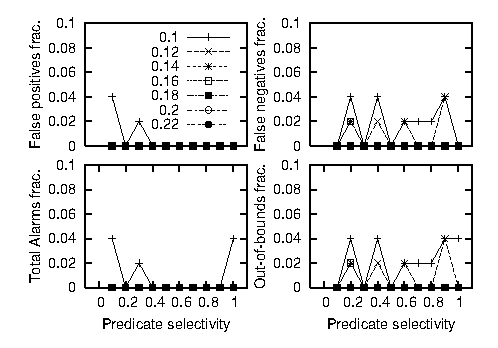
\includegraphics{results/benign}}
\caption{Fraction of alarms, out-of-bounds estimates, alarms for
  in-bounds estimates (false positives) and undetected out-of-bounds
  estimates (false negatives) over all runs for different selectivities ($x$ axis) and
  different $\epsilon$ parameters (one per curve).}
\label{fig:benign}
\vspace*{-2em}
\end{figure}

\begin{figure*}
\centerline{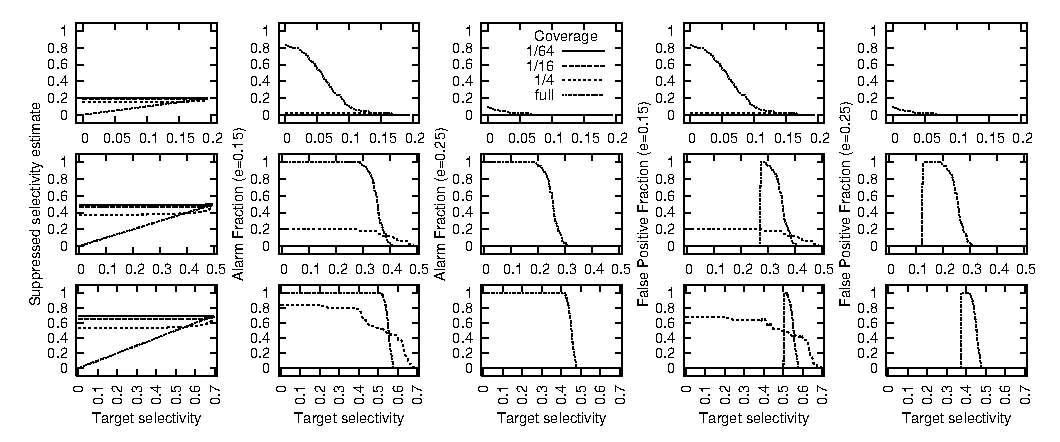
\includegraphics{results/targeted}}
\caption{The effects of the targeted strategy on three predicate polls
  of selectivities $0.2$ (top), $0.5$ (middle), and $0.7$ (bottom).  All
  $x$ axes are the target selectivity of the adversary, from the
  predicate selectivity down to $0$.  On
  the left, we show the average suppressed selectivity.  The next two
  columns show the fraction of alarms over all runs  with an aggressive $\epsilon=0.15$
  and with a more conservative $\epsilon=0.25$.  The final two columns
  show the fraction of false positives over all runs with the same two $\epsilon$ values.
  In each graph, we show different curves for four levels of adversarial
  coverage.}
\label{fig:targeted}
\vspace*{-2em}
\end{figure*}

We raise an alarm when the deflation verification condition fails (for given
$\epsilon$ parameter), and we claim an estimate $\estcpred$
\emph{in bounds} when it satisfies the error bounds of Theorem~\ref{thm:verifcpred}.
Alarms for which the $\estcpred$ estimate was actually in bounds
are conservatively termed \emph{false positives} below, whereas estimates
 that are not in bounds but fail to raise an alarm are termed 
\emph{false negatives}.

In this small scenario,
our approach delivers to the querier no more than $256 \times \lceil \log
10^5 \rceil =
4252$ signed tuples, versus $100,000$ signed tuples via backhauling;
backhauling is preferable only up to a population size of $2,950$. The
ratio of signed-tuple volumes delivered to the querier grows with
$O(U/\log U)$, and more than justifies the $\epsilon=0.15$ verifiable
error bound for our scenario.

\stitle{Benign Behavior.}
We begin with the behavior of \amfm in the absence of adversaries.  We
wish to understand how frequently the deflation verification condition triggers
and when it does, whether it is justified by the occasional outlying
estimate. Figure~\ref{fig:benign} plots the frequency of alarms
and out-of-bounds estimates, as well as the frequency of false positives
and false negatives.

Given the number of sketches (256), the out-of-bounds occurrences are
below 5\% for $\epsilon \geq 0.1$, which is in practice much better
than the worst-case error and confidence probability described above for 256
sketches.  False negatives  are also well below 5\% for all
$\epsilon$ parameters.  Therefore, our
implemented estimators perform well within the worst-case bounds of our
method.  Note that even without the adversary
around, the verification condition does catch some outlier estimates,
especially for high selectivities.  Those appear as alarms that
are not false positives.


\stitle{Targeted Strategy.}
The targeted strategy approximates an adversary who cares about a
particular count suppression, event at the cost of being detected.  She
suppresses as many sketch bits as will cause the estimate (which she
computes locally) to reach the target
count $\cmalicious < \estcpred$. 
When she has limited coverage, her attempts are thwarted as the
remaining, non-malicious aggregators merge their PSRs with those she has
concocted.

Figure~\ref{fig:targeted} explores this strategy for predicate polls of
cardinalities $0.2$, $0.5$, and $0.7$.   Estimates of the selectivity
are affected much more dramatically when the adversary has high coverage
($1/4$-th or more) and otherwise remain fairly close to the actual
selectivity.  However, the dramatic suppressions incurred by the high
coverage adversary necessarily trigger alarms at the querier.  When the
querier applies a tight bound on the verification condition ($\epsilon =
0.15$ in column 2), alarm frequency is greater as the adversary
strives for larger estimate deflation.  Lower-selectivity predicates
(higher rows) suffer less from those alarms, since there is less wiggle
room from our $\epsilon U$ verification condition.

In terms of false positives, the two rightmost columns feature a sharp
drop in the high coverage curves; the $x$-axis point of the sharp drop
off is exactly the lower-bound of Theorem~\ref{thm:verifcpred}.  For
instance, in the bottom right plot, the full coverage false positives
curve drops sharply at target selectivity $\cpred -
\epsilon(U + \cnpred) = 0.7 - 0.25(1 + 0.3) = 0.375$. The top row
(selectivity $0.2$) does not feature this sharp drop off
because the lower bound of our theorem falls below $0$.

Alarm
frequencies are lower for lower coverage, since lower coverage results
in less dramatic estimate deflation; compare the $1/4$-th coverage
curve to the full coverage curve.  Note however that the
$1/4$-th coverage curve does not feature any sharp drops. This is an
artifact of our conservative definition of ``false positives.''  Since
the low-coverage adversary cannot suppress the estimate
significantly, she can suppress it enough to raise an alarm (for the
$0.5$ and $0.7$ selectivities) but not enough to violate a tight error
bound (for $\epsilon=0.15$), causing a false positive.
For the more conservative $\epsilon=0.25$ this is
not the case.



\stitle{Safe Strategy.}
The safe strategy represents an adversary whose primary goal is \emph{not to raise an alarm} while
deflating the count as much as possible.  To do so, the adversary
suppresses sketch bits that do not violate the verification condition
(evaluated as best as possible given the adversary's coverage).  We conservatively
assume for this strategy that the adversary knows her own coverage
exactly, as well as the size of the universe $U$.

Figure~\ref{fig:safeInterior} plots the average deflation bias
introduced by this adversary, under two $\epsilon$ parameters, one very
conservative ($\epsilon = 0.1$) given the number of sketches, and one
more permissive that assumes a relaxed querier ($\epsilon = 0.25$).
(The $X=Y$ line represents the perfect, zero-error, estimate.)
At the tight setting, the adversary does not succeed in biasing the
estimate by more than $\epsilon U$, except under very high coverage, a
quarter of the universe and above.  At the more relaxed $\epsilon$
setting, the adversary hovers around $\epsilon U$ for full universe
coverage, but still remains fairly close to the correct count for lower
coverage values.

Note that, especially when the aggregation topology is beyond the
adversary's control, the ability of the adversary to place herself at
high coverage positions can be kept low.  As a result, the
\emph{expected} deflation bias in this strategy is strongly weighted
towards the low coverage values.  For instance, in a binary tree
topology, half of the aggregators cover only their own PSRs and the
fraction of the value universe corresponding to a single aggregator.




\stitle{Discussion.}
At a high level, our experimental study demonstrates that our
techniques are quite robust: to get near our worst-case bounds
undetected, an adversary needs both to compromise aggregators near the
root of the topology, and to get even luckier than our analysis might
suggest.  The former issue can be mitigated by design; for instance,  by
implementing multiple redundant aggregation trees for the same query.
Furthermore, to remain undetected, the adversary need limit herself to
much lower deflations than those tolerated in the worst-case by our result.
At the same time, our implementation raises interesting issues with respect
to fine-tuning for a real-life 
setting---we are currently exploring different techniques
in that context.

\begin{figure}
  \centerline{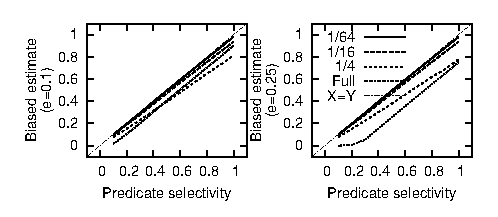
\includegraphics{results/safeInterior}}
  \caption{Average deflated selectivity estimate for an adversary of varying coverage
    (different curves) using the safe interior strategy.  On the left, the
    strategy uses a timid $\epsilon=0.1$.  On the right the
    strategy uses a more permissive $\epsilon=0.25$.}
  \label{fig:safeInterior}
\vspace*{-2em}
\end{figure}


\Section{Conclusions and Future Work}
\vspace*{-1em}
This work on \proofsketches represents a first step in
an agenda towards general-purpose verifiable distributed query processing.
Our approach marries two historically disjoint technologies: cryptographic
authentication and approximate query processing.  While this sounds
complex, our FM-based \proofsketches provide a remarkably simple
defense against the introduction of spurious data during aggregation.
Our complement technique for detecting suppressions is also
simple, though it does require the querier to
track the size of the sensor population.  While
this is quite realistic in a number of important practical settings,
there are scenarios for which alternative suppression
defenses would be welcome. We believe this is an important area for
future research.

\stitle{Acknowledgments} We are grateful to Aydan Yumerefendi for exploring many alternatives to
our approach at an early stage, to David Wagner and Dahlia Malkhi
for their helpful, insightful comments on earlier drafts of this work,
%to Satish Rao for his perspective on $k$-connectivity, 
and to the
anonymous reviewers for the feedback.


%We are optimistic about several potential extensions to this work.
%One direction is to combine our techniques with 
%privacy-preserving query processing, in the hopes of developing a more
%comprehensive notion of trustworthy distributed querying than has been considered
%to date.  Another interesting challenge is to move beyond aggregation
%queries to provide verifiable ``enumerative,'' non-aggregated queries
%-- perhaps to verify approximate~\cite{Babcock2003} or
%``partial''~\cite{Raman2002} results.  Verifiable counts should be a
%key building block in that context.  More generally, we hope to develop more formal
%algebraic characterizations of the ``proof sketchability'' of various
%functions, to understand the bounds of applicability of this idea.




%\Section*{Acknowledgments}
% 

{
\small
%\bibliographystyle{latex8}
%\bibliography{amfmShort}}

\begin{thebibliography}{}\setlength{\itemsep}{-0.5ex}\small

\vspace*{-1em}
\bibitem{AgrawalHaasKiernan2004}
R.~Agrawal, P.~J. Haas, and J.~Kiernan.
\newblock A system for watermarking relational databases.
\newblock In {\em SIGMOD}, 2003.

\bibitem{AgrawalSrikantThomas2005}
R.~Agrawal, R.~Srikant, and D.~Thomas.
\newblock Privacy preserving {OLAP}.
\newblock In {\em SIGMOD}, 2005.

\bibitem{BarYossef2002}
Z.~Bar-Yossef, T.~Jayram, R.~Kumar, D.~Sivakumar, and L.~Trevisan.
\newblock {Counting distinct elements in a data stream}.
\newblock In {\em Proceedings of RANDOM}, 2002.

\bibitem{Bloom1970}
B.~H. Bloom.
\newblock Space/time trade-offs in hash coding with allowable errors.
\newblock {\em Comm. of the ACM}, 13(7), 1970.

\bibitem{Considine2004}
J.~Considine, F.~Li, G.~Kollios, and J.~Byers.
\newblock {Approximate Aggregation Techniques for Sensor Databases}.
\newblock In {\em ICDE}, 2004.

\bibitem{Flajolet1985}
P.~Flajolet and G.~N. Martin.
\newblock {Probabilistic Counting Algorithms for Data Base Applications}.
\newblock {\em JCSS}, 31(2), 1985.

\bibitem{Ganguly2003}
S.~Ganguly, M.~Garofalakis, and R.~Rastogi.
\newblock Processing set expressions over continuous update streams.
\newblock In {\em SIGMOD}, 2003.

\bibitem{Gibbons2001}
P.~B. Gibbons.
\newblock Distinct sampling for highly-accurate answers to distinct values
  queries and event reports.
\newblock In {\em VLDB}, 2001.

\bibitem{Gibbons2001SPAA}
P.~B. Gibbons and S.~Tirthapura.
\newblock Estimating simple functions on the union of data streams.
\newblock In {\em SPAA}, 2001.

\bibitem{Huebsch2004}
R.~Huebsch, B.~N. Chun, J.~M. Hellerstein, B.~T. Loo, P.~Maniatis, T.~Roscoe,
  S.~Shenker, I.~Stoica, and A.~R. Yumerefendi.
\newblock The architecture of {PIER}: an {I}nternet-scale query processor.
\newblock In {\em CIDR}, 2005.

\bibitem{Madden2002}
S.~Madden, M.~J. Franklin, J.~M. Hellerstein, and W.~Hong.
\newblock {TAG}: A {T}iny {AG}gregation service for ad-hoc sensor networks.
\newblock In {\em OSDI}, 2002.

\bibitem{Malkhi2004}
D.~Malkhi, N.~Nisan, B.~Pinkas, and Y.~Sella.
\newblock {Fairplay---A Secure Two-Party Computation System}.
\newblock In {\em USENIX Security}, 2004.

\bibitem{Manjhi2005}
A.~Manjhi, S.~Nath, and P.~B. Gibbons.
\newblock Tributaries and deltas: efficient and robust aggregation in sensor
  network streams.
\newblock In {\em SIGMOD}, 2005.

\bibitem{mm:vldb02}
G.~S. Manku and R.~Motwani.
\newblock {Approximate Frequency Counts over Data Streams}.
\newblock In {\em VLDB}, 2002.

\bibitem{manku:sigmod99}
G.~S. Manku, S.~Rajagopalan, and B.~G. Lindsay.
\newblock {Random sampling techniques for space efficient online computation of
  order statistics of large datasets}.
\newblock In {\em SIGMOD}, 1999.

\bibitem{Przydatek2003}
B.~Przydatek, D.~Song, and A.~Perrig.
\newblock {SIA: Secure Information Aggregation in Sensor Networks}.
\newblock In {\em SenSys}, 2004.

\bibitem{Vitter1985}
J.~S. Vitter.
\newblock Random sampling with a reservoir.
\newblock {\em ACM Transactions on Mathematical Software}, 11(1), 1985.

\bibitem{Wagner2004}
D.~Wagner.
\newblock Resilient aggregation in sensor networks.
\newblock In {\em ACM SASN}, 2004.

\end{thebibliography}

\end{document}



% LocalWords:  HIDs PSR PSRs

%% The below is deprecated text we might want to mine.

% %\begin{figure}
% \begin{eqnarray}
% \mathcal{I}(x) &=& < 2^{b(h(x))}> \;\; ; \;\;\\
% \mathcal{M}(<p>, <q>) &=& <p\ \mathrm{OR}\ q> \;\; ; \;\;\\
% \mathcal{E}(<p>) &=& 2^{f(p)}/0.77351
% \end{eqnarray}
% Some explanation of the notation is called for. $h$ is a hash
% function, and $b$ maps a bit vector to the bit position of its
% lowest-order 1-bit (e.g., $b(0110100) = 2$). $f$ maps a bit vector to the bit position of its
% lowest-order 0-bit (e.g., $f(0110100) = 0$).
% % \label{fig:FM}
% % \end{figure}


% \SubSection{Authentication Manifests for FM (AM-FM)}
% \label{sec:am}
% As for vUNION, we require each PSR component to be attributable to a
% signed input value.  However, in the context of FM-based counts, we
% can utilize a very compact Authentication Manifest: one exemplar for
% each of the $\log n$ bits of the PSR (see Figure~\ref{fig:AM}).
% 
% 
% The initializer produces a PSR of the form $<p, \mathcal{A}_p>$, where
% $p$ is the FM bit vector (as described above), and $\mathcal{A}_p$ is
% the authentication manifest for that bit vector.  The manifest is a
% vector of \emph{support components}, one for every bit position of the
% FM bit vector that is set to 1.  Each support component contains the FM
% bit position $i$ to which it corresponds,  a
% sensor value $x$, the originating data source $a$ for that value, and a
% signature $s_a(x)$ on $x$ by $a$.  A verifier can check the validity of
% a PSR by ensuring that for every FM bit vector position $i$, that bit is
% set to 1 if and only if the signed
% value $x$ would indeed set that FM bit position to 1 (i.e., if and only
% if $i = b(h(x))$).  Components in the manifest corresponding to 0-bit
% positions of the FM bit vector are empty.
% 
% Given two PSRs, the merger function $\mathcal{M}$ forms the bitwise OR
% of their FM bit vectors, and uses the same $\sqcup$ operator as vUNION
% to form the set union of exemplars, one per bit of the FM sketch.
% 
% Given a PSR $<p, \mathcal{A}_p>$, the evaluator $\mathcal{E}$ produces
% an approximate COUNT $\hat{c}$ as per the standard FM logic (in the
% specific scheme, $\hat{c} = 2^{f(p)}/0.77351$) if the manifest
% $\mathcal{A}_p$ is valid given the bit vector $p$, and $\mathit{error}$
% otherwise.
% 



% \SubSection{Omission Protection: Yes/No Counting}
% \label{sec:YesNo}
% 
% Having protected \amfm sketches from spurious setting of bits, we now
% turn to protecting them from spurious resetting of bits, that is,
% adversarial crimes of omission.
% 
% In the terminology of Gray~\cite{Gray1996} and TAG~\cite{Madden2002},
% FM sketching is an Algebraic aggregate, with PSR size that is
% independent of the input data (dependent only on the data \emph{%   domain}).  More importantly, as observed by Considine, et
% al.~\cite{Considine2004} (and expanded upon in~\cite{Nath2004}), FM
% sketches are \emph{duplicate-insensitive}, hence amenable to the
% multipath omission protection scheme.
% 
% MOP alone -- even if it were feasible -- would not be sufficient to
% guarantee verifiable aggregation, as it does not protect against an
% adversary ``turning on bits'' during merging or final evaluation.  At
% the extreme, an adversarial aggregator can incorrectly return $2^x-1$
% when it invokes $\mathcal{M}$ on any inputs, effectively ensuring that
% the final estimate returned by $\mathcal{E}$ will be on the order of
% $2^x$ regardless of the number of input data.
% 
% 
% 
% \comm{MNG}{We need to be a little careful here wrt the development in the
% UNION section: there, it seems like we're talking about estimating the number
% of distinct measurement values, whereas here we're talking about the number of
% generators. The technique would of course also work if we knew the exact number
% of distinct values, but I'm not sure how we'd get that...}










\pagebreak
\appendix

The old text

\Section{Introduction}
\comm{J}{This was the VLDB outline, so needs to be reworked for CCS.}

\comm{J}{Setup: Distributed query processing in many new settings.  Give
examples from web svcs a la Agrawal, sensornets, p2p.  A key change
is the participation of multiple parties, either explicitly or via
security breaches.  Security and trust now a concern.}


\comm{J}{Problem setup}
In this paper we consider the problem of ensuring verifiable,
efficient, approximately correct results to typical distributed
multi-party aggregations.  We begin by carefully defining the problem
we are addressing in terms of a threat model that includes two basic
forms of misbehavior: inaccurate reporting of base data, and incorrect
computation of intermediate aggregate results.

\comm{J}{Contributions of paper}
Given this problem statement, there are two main constructive
contributions to this paper: one specific technique to address the
problem, and a general treatment of the solution that situates it in
the design space of extensible aggregation.

\comm{J}{\amfm}
We present an extension to Flajolet-Martin sketches that is robust to
tampering of two sorts: mis-reporting of input data, and tampering
with the running state of the aggregate.  Our solution provides a \emph{compact signature} for the aggregate result that can be verified
completely in logarithmic checks, and verified in an incrementally
refined manner for approximate checks.  

\comm{J}{Generalization and API}
In addition to presenting a specific solution for the problem, we
highlight the fundamental properties of our scheme that make it
verifiable and efficient to compute and check; this can be exploited
via simple extensions to a typical extensible aggregation interface.

\SubSection{Structure of the Paper}


\Section{MIN: A Simple Motivating Example}
In this section we consider the problem of designing a verifiable MIN
aggregate in this setting.  As we will see, the MIN aggregate has a
suite of properties that make it very easy to secure.

First, consider the trio of functions for the MIN aggregate:
\begin{eqnarray}
\mathcal{I}(x) &=& <x>\\
\mathcal{M}(<x>, <y>) &=& min(x,y)\\
\mathcal{E}(<x>) &=& x
\end{eqnarray}
Note that the result of the MIN aggregate is equal to one of the
original input data values; this makes MIN an \emph{exemplary}
aggregate in the TAG terminology~\cite{Madden2002}.  An additional important
aggregate property of MIN pointed out in TAG is that it is
\emph{duplicate-insensitive}: regardless of how many copies of each
input value is submitted to the aggregate, the result of the MIN
function will be the same.

This suggests a very simple enhancement to MIN to improve the
verifiability of the computation in the network.  First, we require
that input data values be accompanied by PKI signatures from their
data sources.  Given input data pairs of the form $<\mathit{value},
\mathit{source}, \mathit{signature}>$, we define the verifiable MIN
(VMIN) aggregate in Figure~\ref{fig:vmin}.
\begin{figure*}
\begin{eqnarray}
\mathcal{I}(x,a) &=& <x,a,s_a(x)>\\
\mathcal{M}(<x,a,s_a(x)>, <y,b,s_b(y)>) &=&
\left\{\begin{array}{l}
<x,a,s_a(x)>, \mathit{if\ } x = \min (x, y)\\
<y,b,s_b(y)>, \mathit{otherwise} 
\end{array}\right.\\
\mathcal{E}(<x,a,s_a(x)>) &=& <x,a,s_a(x)>
\end{eqnarray}
\caption{Definition of VMIN.}
\label{fig:vmin}
\end{figure*}

This is still an exemplary aggregate.  Note that there can be \emph{collisions} in which two or more nodes both have the minimal value;
in this case, the signature on the final result is non-deterministic,
depending on the arrival time of the different PSRs to be merged, and
the way in which ties are broken during merging.  Regardless of the
number of collisions or the way they are handled, the actual minimum
value produced is the same, and in that respect the minimum that is
computed is deterministic, and also duplicate-insensitive.

Now, when a client querier receives a result from vUNION, it can in a
single check verify that the result was produced by a sensor
registered with the PKI. \comm{J}{Petros: can we add early commitment
  to this somehow?}  This simple check protects against spurious data,
spurious PSRs, PSR manipulation and finalization attacks.  It does not
protect against suppression of either input data or PSRs, however.

\SubSection{Handling Suppression for Verifiable MIN}
To prevent suppression, we can rely on one of two schemes.  The first
scheme simply uses redundant communication to attempt to route around
agents of suppression; the second is more efficient but relies upon
knowing a stable population of participants in the network.

\subsubsection{Multipath routing}
As noted in the TAG paper, duplicate-insensitive aggregates can be
robustly computed in the face of loss or explicit suppression via \emph{multi-path routing} of PSRs in the network.  In essence, PSRs can be
redundantly routed and merged within the network, and due to
duplicate insensitivity this does not perturb the final answer.  With
our VMIN aggregate, note again that we are most interested in the true
MIN \emph{value}, but any exemplar of the true MIN is equivalent, and
only one needs to propagate through the network for the correct MIN
value to emerge.

The resilience of this scheme to attack depends upon the topology of
the forwarding network, and the ability of an adversary to place
itself at various places within that topology.  For example, one can
implement an exhaustive flooding-based scheme in which each node sends
its PSR to be aggregated by all neighbors it has not previously heard
from.  Suppressing the true aggregate in this setting would require
the adversary to control enough forwarding nodes to partition the
network so that all sensors with the true MIN value are separated from
the evaluator.   By contrast, a gossip scheme (e.g., \cite{Demers1987}) will have
each node choose a subset of its neighbors at random and send its PSR
to it.  Considine et al.~\cite{Considine2004} and Nath et
al.~\cite{Nath2004} propose a similar technique that takes advantage of
a wireless broadcast medium to organize nodes in \emph{concentric rings}
of increasing logical distance from the aggregation requestor. A node in
ring $i$ can obtain a PSR by listening to transmissions originating from
any node in ring $i+1$.


\comm{J}{analysis depends on topology. can we toss off any theory results
  here on the relationship between number of graph partitions and topology?}
The worst-case analysis of an adversary's power corresponds directly
to its ability to intercept packets on all routes from data sources to
the proxy node.  This is a well-studied network topology design
problem \comm{J}{find citations}, and the adversary's ability to suppress
messages can be tightly bound based on the connection topology of the
network and the number (or distribution) of colluding nodes
compromised by the adversary.  We will return to these issues in more
detail in the next section.  \comm{J}{We will???}

The alternative to 

Of course in the unhappy scenario that the true
minimum is suppressed or lost on all paths, the error introduced is
unbounded (in the absence of information about the data distribution).
This is not a weaknesses of our scheme here per se, it is a property
of the MIN aggregate being inapproximable on partial inputs.  

\subsubsection{Roll Call}
In this section we present a ``roll call'' scheme that can assure the
querier that a specific set of data sources have indeed contributed to
the answer.  \comm{J}{Beware of previous sentence.  Maybe we can only
guarantee the number of data sources!}

\subsubsection{Discussion}
At this point, we have shown that MIN can be secured by the
combination of a simple signature and either multi-path routing or
simple counting of participants.  Indeed, this analysis extends to any
exemplary, duplicate-insensitive aggregate function, including rank
aggregates like MIN, MAX, and TOP-K.  We note in passing that not all
exemplary aggregates are duplicate-insensitive: MODE and MEDIAN are
two counter-examples, being exemplary but sensitive to duplicates,
though MEDIAN DISTINCT (i.e., the median of all distinct values) is
both exemplary and duplicate-insensitive, hence amenable to our simple
scheme here.






\subsubsection{Defenses}
\label{sec:defenses}

Authentication manifests prevent adversaries effectively from injecting
spurious data or their \emph{derivatives} into the system.  Suppression
of data, however, is not significantly hindered by AM.  We explain
below.

An authentication manifest cannot contain spurious data, that is, data
that no generator has signed.  Any PSR with such an authentication
manifest would be rejected by correct aggregators, since either the
signature accompanying the data value would not correspond to a data
generator, or because no valid signature for the data value in question
would appear in the manifest.  Recall that a collusion of a malicious
sensor with a data generator to legitimately sign an incorrect raw data
value does not constitute a threat in our setting; we wish to aggregate
whatever a legitimate sensor has endorsed, and any checks for
the correctness of sensors or generators falls out of the scope of our threat
model.  For these reasons, spurious data values cannot be introduced at
any stage of the aggregation (vulnerabilities 2-4 in
Figure~\ref{fig:setup}). \comm{JMH}{If we include this paragraph, we
  should be careful about what is the role of generator vs. sensor.}

Since any PSR considered by a correct aggregator or the finalizer can
contain only correct data values in its authentication manifest, then
no adversarial aggregator in the system can affect the result
by introducing spurious data, at any point in the aggregation.  Spurious
data would affect an FM bitvector by turning on a bit that was
previously off, thereby potentially inflating the result of the
evaluator function $\mathcal{E}$ (in Equation~\ref{eqn:AMFM-E},
setting to 1 bits that were previously set to 0 can push the position of
the first 0-bit higher, thereby increasing the exponent $f(p)$,
which would also increases the count estimate by some power of 2).
However, a correct aggregator or
finalizer verifies any 1-bit in the FM
bitvector, by finding in the accompanying authentication manifest a
supporting, signed data value coming from a sensor.  If a bit is
turned on due to a spurious data value, but can be supported by a
correct data value, then the introduction of the spurious data value has
had \emph{no effect} in the aggregation.

Through the same line of reasoning, no PSR manipulation can inflate the
final result of FM-based probabilistic counting.  Unless a bitvector
1-bit is supported by a correct data value in some authentication
manifest, the bitvector will be rejected by any correct aggregator or
finalizer.  If some supporting, correct data value exists for a
bitvector position originally turned on by malicious PSR manipulation,
then the manipulation had no effect, since the correct data value would
have eventually turned on the appropriate bit anyway.

However, authentication manifests do not prevent a malicious sensor from
suppressing data values: such a sensor can just ignore a particular data
value, leaving the corresponding bitvector bit in the off state, and
keeping the corresponding component of the authentication manifest
empty.  Similarly, a malicious aggregator can suppress some 1-bits and
their corresponding supports from its inputs, incorrectly leaving some
output bitvector bit positions in the off state.  Such suppression of
data or PSR bits can lead to result deflation (again, if the position of
the lowest-order 0-bit in the FM bitvector were pushed lower, then the
exponent $f(p)$ in Equation~\ref{eqn:AMFM-E} would decrease, thereby
decreasing the count estimate by some power of 2).  We describe two
methods of preventing or counteracting suppressions, via YES/NO counting
when the number of all data generators is known
(Section~\ref{sec:YesNo}), or via redundant path routing when this
number is unknown (Section~\ref{sec:redundantPath}).





\SubSection{Multipath Routing}
\label{sec:redundantPath}

When the size $N$ of the population is unknown, the Yes/No counting
technique from Section~\ref{sec:YesNo} is not immediately applicable.
A more generally applicable technique for addressing suppression is
required.  Since \amfm is an 
\emph{order- and duplicate-insensitive} correct
aggregate~\cite{Nath2004}, we can use multipath routing as a more
drastic defense against suppression.  In this section we prove that
\amfm is ODI-correct.

Briefly, an aggregate is ODI correct if an only if its initializer
$\mathcal{I}$ preserves duplicates, and its merge function $\mathcal{M}$
is commutative, associative, and same-synopsis idempotent.  The FM
portion of \amfm is shown to be ODI correct by Nath et al.~\cite[Claim
1]{Nath2004}. Here, we expand that earlier proof to take into account
the authentication manifest portion of \amfm.

\begin{theorem}
\amfm is ODI-correct.
\end{theorem}








\SubSection{Validating AM-FM Transmissions}
Given an FM sketch and an AM array, it only requires $\log |D|$ checks
to ensure that the sketch was not tampered with via spurious data, PSR
manipulation or finalization attacks.  Again, suppression attacks are
not prevented in this way, but can be addressed via multi-path routing.


\SubSection{\amfm Networking}
\comm{J}{Talk here about multi-path.  Introduce Y/N/Count and RollCall
  approaches.  Provide a couple examples of multi-path techniques and
  suppression analyses.}

\SubSection{Extensions}
Other aggs (e.g., AVG).  Check Considine/Nath.

Note tricks that FM gives us for free.  E.g., distributed sampling.
What else?  Watch Gibbons papers and check citeseer citations of FM.

\Section{Extensibility}

\Section{Conclusion}

\balancecolumns



\SubSection{UNION: A Simple Example}
\label{sec:vUnion}

To introduce the basic ideas used in \proofsketches, we begin with a
simplistic aggregation function, UNION, which forms the set
(``distinct'') union of all input data, and returns that set as a
single complex object.  UNION is not a particularly natural
aggregation function, and strict relational systems would not support
it.  But it serves as a very simple and general example for our
initial discussion (and is relevant to systems built on nested data
models like objects or XML.)  Given a verifiable scheme for a
multi-party UNION, in Section~\ref{sec:template} we will be able to
give a general template for constructing verifiable aggregation
functions, which we will use later in the paper to derive a broad
collection of useful aggregates.

First, consider the trio of functions for a simple UNION aggregate
% \footnote{UNION is not a particularly useful aggregate, and it breaks
%   the pure relational model.  We discuss it here for expository
%   purposes, since verifying it is fairly simple. More practical but
%   complex verifiable aggregates are given below.  However, we note
%   that the (v)UNION example as given here can be used directly in an
%   extended data model like that of SQL99 or XML, or it can be modified
%   to a pure relational implementation that represents a set as a text
%   string that is opaque to the query language\cite{darwendate}.}:
\[\mathcal{I}(x) = \{x\} \;\;;\;\; \mathcal{M}(S, T) = S \cup T \;\;;
\;\; \mathcal{E}(S) = S\]

UNION can be perturbed in two possible ways: via the insertion of
spurious values that should not be in the answer, and via the
suppression of values that should be in the answer.  We refer to these
as crimes of ``commission'' and ``omission'' respectively.  Commission
protection ensures that the computed aggregate is a \emph{lower bound}
(i.e., a subset) of the true answer.  Omission protection ensures that
the computed aggregate is an \emph{upper bound} (i.e., a superset) of
the true answer.  The combination provides the desired verifiability.
We proceed to discuss each in turn.

\SubSection{Commission Protection with Authentication Manifests}
\label{sec:am}
To protect against comission attacks, we simply require that all raw
data values be accompanied by PKI signatures from their associated
data generators (Figure~\ref{fig:setup}).  This means that the input
to the Initializer function is now a triple $(x, a, s_a(x))$, and PSRs
are of the form$\{(x, a, s_a(x))\}$, where $x$ is a value to be
aggregated, $a$ is the identity of the sensor for $x$, and $s_a(x)$ is
the result of signing $x$ with $a$'s private key.  The only detail to
be addressed is to ensure that the merging function computes a proper
set-union of values, which removes duplicate instances of a value $x$
(possibly signed by different parties).  This is complicated by the
fact that each copy of a value $x$ is now distinguished by its
generator and signature.  To preserve the intention of the original
UNION aggregate, we do not care which signed ``exemplar'' of the value
$x$ is preserved.  However, the choice should be handled in such a
way that the merging function remains commutative and associative.
One reasonable way to solve this is to choose the exemplar for $x$
whose signature has the largest value (interpreted as an integer).
But any total ordering scheme $\prec$ on exemplars will do.

As a matter of notation, we define the operator $\sqcup$ to be
the set union over signed values that chooses exemplars according to some
total order $\prec$ on exemplars.  We define a new version of the
UNION aggregate, vUNION, as follows:

\[\mathcal{I}((x, a,s_a(x))) = \{(x, a,s_a(x))\} \;\; ; \;\;
\mathcal{M}(S, T) = S \sqcup T \;\; ; \;\;
\mathcal{E}(S) = S\]

\comm{JMH}{Commented inline is a more formal presentation of vUNION,
  and a proof that its merging function is commutative and
  associative, but I think the above is sufficient.  No?  Should we
  make a TR version that has the commented stuff?}

%% Before presenting details of the verifiable UNION aggregate, we define
%% a useful relational operator:
%% 
%% \begin{defn}
%% Given a relation $R$ whose schema is a set of attributes $A=\{a_1,
%% \ldots, a_n\}$, and a total order $\prec_B$ over the attributes $B
%% \subset A$, we define the \emph{relational argmax} operator $\Gamma$ to
%% choose for each distinct value on attributes in $A-B$ (each group) a
%% tuple with the maximal value according to $\prec_B$, i.e.:
%% \[ \Gamma(\prec_B, R) = \{t \in R | \forall s \ne t \in R
%% ((\forall i \in A-B \; t.i = s.i) \Rightarrow  s \prec_B t)\}\]
%% \end{defn}
%% As a notational convenience, we will sometimes write $\Gamma_B(R)$ as
%% shorthand for $\Gamma(\prec_B, R)$ when the specific total order is
%% not of interest.
%% 
%% Given this definition, we specify the verifiable UNION (vUNION)
%% aggregate over such data as
%% %in Figure~\ref{fig:vUnion}.
%% %\begin{figure*}
%% \begin{eqnarray}
%% \mathcal{I}(x,a,s_a(x)) &=& \{(x,a,s_a(x))\}\\
%% \mathcal{M}(S, T) &=& \Gamma(\prec_{\{a,s_a(x)\}},S \cup T)\\
%% \mathcal{E}(S) &=& S
%% \end{eqnarray}
%% 
%% % \caption{Definition of vUNION.}
%% % \label{fig:vUnion}
%% % \end{figure*}
%% We briefly demonstrate that the merging function for the vUNION
%% aggregate is commutative and associative, as required.
%% 
%% \begin{lemma}
%% The merging function $\mathcal{M}(S,T) = \Gamma(\prec_{\{a,s_a(x)\}},S
%% \cup T)$ is commutative and associative.
%% \end{lemma}
%% To show this, observe that $\Gamma$ can be lifted out of unions.
%% I.e.,
%% \[\Gamma_B((\Gamma_B(R) \cup  \Gamma_B(S))) = \Gamma_B(R \cup S)\]
%% This follows directly from $\Gamma_B$ being defined over a total order
%% $\prec_B$.  Given this property, any sequence of merging function
%% applications can be rewritten equivalently as a sequence of set unions
%% with only a single $\Gamma_B$ as the final step.  Since set union is
%% commutative and associative, it follows that $\mathcal{M}$ is as well.
%% \newqed

The final result of the vUNION includes not only an aggregate result
(the distinct $x$'s), but also a signed exemplar for each value.  We
refer to the set of exemplars as an \emph{authentication manifest} for
the aggregate result: a listing of ``witnesses'' that can be used to
verify the desired result.  A verifier can check the validity of a PSR
by ensuring that for each exemplar $(x, a, s_a(x))$, the public key of
$a$ (available from the PKI) produces the correct value of $x$, i.e.
$pk_a(s_a(x)) = x$.  Assuming all data generators are properly
certified and trusted, the vUNION authentication manifest directly
prevents the injection of spurious data into PSRs at any step of the
aggregation.  \comm{JMH}{Map properly to the Figure}. Moreover, it
allows such comission attacks to be identified early by intermediate
aggregation agents, which can optionally check the authenticity of
signed inputs. \comm{JMH}{We should postpone the previous sentence to
  the section on accountability.}

% If aggregation agents or
% finalizers have access to a sensor agent's private key (e.g., they are
% on a machine that plays multiple roles), the benefit is a bit more
% subtle, since partcipiating nodes can introduce signed, spurious data
% at any stage.  Of course, each node is ``on the record'' for any value
% that they sign, so periodic auditing or spot-checking of results could
% help discourage commission attacks.  Moreover, in some cases,
% additional invariants help to discourage authenticated spurious data.
% For example, in many queries each node should produce only one value
% for a query; this is a common case for monitoring queries about the
% nodes in the system (e.g., the count of live nodes, the average
% resource availability on a node, etc.)  In these scenarios, an
% aggregator can introduce only one spurious value without being
% detected, and this value must represent its \emph{own} state. It cannot
% ``bear false witness'' to the state of other nodes.
% 


\SubSection{Omission Protection}
The authentication manifest of vUNION prevents the injection of
spurious data, but provides no protection against omission attacks
that suppress either data or PSRs. We now present two different
solutions to those problems.



% 
% 
% 
% For example, one
% can implement an exhaustive flooding-based scheme in which each node
% sends its PSR to be aggregated by all neighbors it has not previously
% heard from.  Suppressing the true aggregate in this setting would
% require the adversary to control enough forwarding nodes to partition
% the network so that all participants with the true MIN value are
% separated from the evaluator.  By contrast, a gossip scheme (e.g.,
% \cite{Demers1987}) will have each node choose a subset of its
% neighbors at random and send its PSR to it.  Considine et
% al.~\cite{Considine2004} and Nath et al.~\cite{Nath2004} propose a
% similar technique that takes advantage of a wireless broadcast medium
% to organize nodes in \emph{concentric rings} of increasing logical
% distance from the aggregation requestor. A node in ring $i$ can obtain
% a PSR by listening to transmissions originating from any node in ring
% $i+1$.
% 
% 
% 
% \comm{J}{analysis depends on topology. can we toss off any theory results
%   here on the relationship between number of graph partitions and topology?}
% The worst-case analysis of an adversary's power corresponds directly
% to its ability to intercept packets on all routes from data sources to
% the proxy node.  This is a well-studied network topology design
% problem \comm{J}{find citations}, and the adversary's ability to suppress
% messages can be tightly bound based on the connection topology of the
% network and the number (or distribution) of colluding nodes
% compromised by the adversary.  We will return to these issues in more
% detail in the next section.  \comm{J}{We will???}

% Unfortunately, in practice it can be difficult to ensure a network
% topology that is regular enough to 
% Of course in the unhappy scenario that the true
% minimum is suppressed or lost on all paths, the error introduced is
% unbounded (in the absence of information about the data distribution).
% This is not a weaknesses of our scheme here per se, it is a property
% of the MIN aggregate being inapproximable on partial inputs.  

\subsubsection{Complementary Omission Protection(COP)}
\label{sec:cop}
Rather than relying on properties of the network topology, in this
scheme we rely on the querier \emph{already} knowing an aggregation
result for the full distributed data set, but not for queries with
selection predicates that eliminate tuples.  To prevent omission
attacks in this scenario, we will require explicit processing of the
\emph{complement} of the query predicates; hence we refer to this
approach as \emph{Complementary Omission Protection (COP).}  We proceed
to describe this for our verifiable UNION aggregate.

Let $U$ be the set of distinct data values in the network at the time
of the query; we assume the querier knows the value of the aggregate
over $U$, i.e., $\mbox{UNION}(U)$.  In order to provide an upper bound
for an aggregation/selection query $\mbox{UNION}(\sigma_p(U))$, we
rewrite the query to compute both $P = \mbox{vUNION}(\sigma_p(U))$ and
$\overline{P} = \mbox{vUNION}(\sigma_{\neg p}(U))$.  The querier can
verify that each element of $P$ and $\overline{P}$ is properly signed
and in the proper result set (i.e., it should be in $P$ iff it
satisfies $p$).  Since it knows $\mbox{UNION}(U)$, the querier can
also check that $\pi_x(P \cup \overline{P}) = \mbox{UNION}(U)$ --
i.e., each distinct data value in the network was reported.

In essence, the COP technique uses a closed-world assumption and
detects omissions by requiring the entire world to be ``covered'' by
the results returned to the querier.  Now clearly in this simplistic
scenario of a UNION aggregate, this technique is artificial: if we
really knew the complex object $\mbox{UNION}(U)$ at the querier, we
would be able to compute the set $U$, and hence could have evaluated
the query without any distributed computation!  However, we will soon
generalize this technique to more compact aggregates than UNION, which
are not amenable to centralized querying.

Another natural objection to this approach is the need for the querier
to maintain even a compact aggregate result on the full data set over
time.  This can be expensive if the data is changing, especially since
this aggregate must be maintained in a verifiable manner.  In the next
section we will discuss the use of approximate aggregate maintenance
that can relieve this burden.

\comm{JMH}{The following paragraph is bunk.  With many duplicates, the
  UNION will not cover all the nodes in the network.}  While this
objection is valid in general, it does not hold in all cases.  One
important special case arises frequently in distributed systems:
queries where there is exactly one value per data generator at any
time.  In that case, we can check that the union of signatures
obtained in $P$ and $\overline{P}$ covers all the nodes in the
network.  \comm{JMH}{This is not what I said above: knowing the result
  of the AGGREGATE on $U$ in advance!}  This is the model for all
queries in the TinyDB/TAG model for epoch-based querying of physical
sensors~\cite{Madden2002}.  It also occurs analogously in distributed system
monitoring scenarios, where it is common to maintain the values of
some metrics (load, uptime, etc.) at each end-system, one value per
metric per system at each time.


----

\SubSection{Multipath Omission Protection (MOP)}
\label{sec:mop}
The \proofsketches we develop here are \emph{duplicate-insensitive}
aggregates~\cite{Madden2002,Considine2004,Nath2004}

 like MIN and MAX
may be copied and redundantly routed through multiple paths in a
network, without requiring any bookkeeping to remove duplicate
messages in order to correctly evaluate the final result.  A variety
of techniques have exploited this property to mitigate the effects of
communication failure during distributed aggregate computation.  Our
vUNION aggregate is duplicate-insensitive: its merging function
chooses the same exemplar for a value $x$ regardless of the number of
times each exemplar is merged in.  Hence multipath routing is one
possible strategy for preventing omission attacks on vUNION.  We refer
to this approach as \emph{Multipath Omission Protection (MOP).}

While the direction is encouraging, multipath routing has not been
explored in an adversarial setting for distributed aggregation, and
provides no guarantees on avoiding determined
adversaries.\comm{JMH}{Double-check that assertion!}  How do we
guarantee that the network topology is robust against adversaries?  

All of the \proofsketches we present in this paper are
duplicate-insensitive, and are amenable to MOP.  However, since the
state of the art with respect to adversary-proof multipath routing has
limitations, we now explore an additional protection against omission,
which works under a different set of conditions.

